\chapter{equazioni differenziali}
\label{ch:edo}

\section{classificazione}

Le equazioni differenziali sono una classe di \emph{equazioni funzionali}
\mynote{equazioni funzionali}
\index{equazione!funzionale}
ovvero
equazioni in cui l'incognita non è un numero (come accade nelle equazioni algebriche) ma è una funzione. La funzione incognita $u$, sarà quindi funzione di una variabile indipendente $u=u(x)$.
Ad esempio $u$ potrebbe essere la traiettoria di un proiettile che descrive la posizione nello spazio in funzione del tempo $x$. Se nelle equazioni algebriche il nome di gran lunga più utilizzato per l'incognita è $x$, nelle equazioni funzionali a seconda dei contesti le convenzioni possono cambiare in maniera drastica. Si dovrà utilizzare un nome per la funzione e un nome per la sua variabile indipendente: $x=x(t)$, $y=y(x)$, $y=y(t)$, $u=u(x)$ sono alcune delle scelte più utilizzate.
Se l'incognita è una funzione $u=u(x)$ le operazioni che possono comparire nell'equazioni sono,
oltre le usuali operazioni algebriche che agiscono sui singoli valori $u(x)$ della funzione,
anche operatori che agiscono sulla funzione $u$ in sé.
Se l'equazione funzionale oltre alle operazioni algebriche comprende anche
l'operatore derivata, si dirà che è una \mynote{equazione differenziale}%
\index{equazione!differenziale}
\emph{equazione differenziale}.
Di contro ci potranno ad esempio essere equazioni che coinvolgono l'operatore integrale e si chiameranno
\emph{equazioni integrali}.

Ci sono quindi diversi concetti che possono aiutare a classificare le equazioni differenziali.
Innanzitutto supporremo sempre che le nostre equazioni siano \myemph{senza ritardo}
(o \emph{senza memoria})
cioè che la funzione $u$ e le sue derivate $u'$, $u''$\dots,
vengano tutte calcolate nello stesso punto $x$.
In caso contrario si parla di
equazioni \emph{differenziali funzionali} (in particolare \emph{equazioni con ritardo}
perché le derivate dipendono tipicamente dai valori assunti nel passato),
argomento che non toccheremo.

Se la funzione incognita è funzione di una singola variabile si dirà che l'equazione è una
\emph{equazione differenziale ordinaria}
\mynote{ODE}%
\index{equazione!differenziale!ordinaria}%
(abbreviato
\emph{EDO} \index{EDO}%
in italiano,
\emph{ODE} \index{ODE}%
per gli anglosassoni).
Di contro se la funzione incognita è funzione di più variabili l'equazione si chiamerà
\emph{equazione differenziale alle derivate parziali}
\mynote{PDE}%
\index{equazione!differenziale!alle derivate parziali}%
 (abbreviato \emph{EDP} \index{EDP} in italiano e \emph{PDE}
 \index{PDE} in lingua inglese).
In questo corso, centrato sulle funzioni di una variabile, tratteremo quindi solamente le equazioni differenziali ordinarie.
L'\emph{ordine}
\mynote{ordine}%
\index{ordine!equazione differenziale}%
\index{equazione!differenziale!ordine}%
dell'equazione differenziale è il numero massimo di derivate successive che vengono applicate alla funzione incognita.
La funzione $u$ sarà definita su un intervallo $I$ della retta reale: $u\colon I \to \RR$
e la funzione e le derivate vengono tutte valutate nello stesso punto. In tal caso
la forma più generale di equazione differenziale ordinaria di ordine $n$ si potrà dunque scrivere come:
\begin{equation}\label{eq:3784643}
  F(x,u(x),u'(x),u''(x), \dots, u^{(n)}(x)) = 0
\end{equation}
con $F\colon \Omega \to \RR$ una funzione data, definita su un insieme $\Omega \subset I\times \RR^{n+1}$.
Una funzione $u\colon I \to \RR$ si dice essere una \emph{soluzione
dell'equazione differenziale} \eqref{eq:3784643} se $u$ è derivabile almeno
$n$ volte in ogni punto $x\in I$ e se \eqref{eq:3784643} è soddisfatta
per ogni $x\in I$.

Usualmente si tende a semplificare la notazione evitando di scrivere sempre
esplicitamente il punto $x$ in cui viene calcolata la funzione.
Sarà quindi usuale
scrivere l'equazione \eqref{eq:3784643}
nella forma abbreviata:
\[
  F(x,u,u',u'', \dots, u^{(n)}) = 0
\]
rendendo anche più evidente il fatto che l'incognita è $u$,
l'intera funzione, e non un singolo valore $u(x)$.


Se ad esempio scegliamo $n=2$ e $F(x,u,v,z)= z+\sin u + v$ otteniamo l'equazione differenziale:
\begin{equation}\label{eq:39872}
 u''(x) + \sin u(x) + u'(x) = 0
\end{equation}
che, in opportune unità di misura, è l'equazione del moto di un pendolo smorzato,
dove $x$ rappresenta il tempo e $u$ la misura dell'angolo di inclinazione del
pendolo rispetto alla verticale.
Osserviamo che nell'esempio precedente la funzione $F$ non dipende direttamente
dalla variabile $x$. Equazioni con questa proprietà si dicono
\emph{equazioni autonome}
\mynote{equazioni autonome}
\index{equazione!differenziale!autonoma}
ed è immediato osservare che se $u(x)$ è soluzione anche una sua traslazione
temporale $v(x) = u(x-x_0)$ è soluzione dell'equazione
(il moto del pendolo non dipende dall'ora in cui si svolge).

Una equazione scritta nella forma \eqref{eq:3784643} si dice \emph{equazione in forma implicita}
\mynote{equazione in forma implicita}%
\index{equazione!differenziale!in forma implicita}%
e per analogia con le equazioni algebriche (si pensi all'equazione
$u^2(x) + x^2 = 1$) ci si aspetta che le soluzioni di tale equazioni siano
meglio rappresentate da curve piuttosto che da grafici di funzione.
Risulta in effetti che la teoria delle equazioni differenziali si applica con
molta maggiore efficacia alle \emph{equazioni in forma normale}
\mynote{equazioni in forma normale}
\index{equazione!differenziale!in forma normale}
che sono le equazioni differenziali di ordine $n$ che possono essere scritte
esplicitando la dipendenza dalla derivata di ordine massimo:
\begin{equation}\label{eq:366793}
 u^{(n)}(x) = f(x, u(x), u'(x), \dots, u^{n-1}(x))
\end{equation}
dove $f\colon \Omega \to \RR$ è una funzione definita su $\Omega\subset I\times \RR^n$.
L'equazione del pendolo si può scrivere in questa forma,
scegliendo $f(x,u,v) = -\sin u - v$.

Più in generale potremmo considerare
\emph{sistemi di equazioni differenziali}
\mynote{sistemi}%
\index{sistemi di equazioni differenziali}%
\index{equazione!differenziale!sistema}%
in più incognite.
Possiamo rappresentare un sistema di $k$ equazioni ordinarie in $m$ incognite nella forma:
\begin{equation}\label{eq:375456}
  \vec F(x, \vec u(x), \vec u'(x), \dots, \vec u^{n}(x)) = \vec 0
\end{equation}
dove $\vec u$ è una funzione $\vec u \colon I \to \RR^m$ le cui componenti sono
le $m$ funzioni incognite:
\[
  \vec u(x) = (u_1(x), \dots, u_m(x))
\]
mentre la funzione $\vec F \colon I \times (\RR^m)^{n+1} \to \RR^k$ è stavolta
una funzione a valori vettoriali $\vec F = (F_1, \dots, F_k)$ cosicché l'equazione vettoriale
\eqref{eq:375456} è effettivamente equivalente ad un sistema di $k$ equazioni:
\[
\begin{cases}
F_1(x,\vec u(x), \vec u'(x)\dots, \vec u^{(n)}(x)) = 0\\
F_2(x,\vec u(x), \vec u'(x)\dots, \vec u^{(n)}(x)) = 0\\
\quad\vdots \\
F_k(x,\vec u(x), \vec u'(x)\dots, \vec u^{(n)}(x)) = 0\\
\end{cases}
\]
Vedremo che per le equazioni ordinarie del primo ordine è naturale,
come accade per le equazioni algebriche,
avere lo stesso numero di equazioni e di incognite dunque è tipico avere singole
equazioni scalari del primo ordine
(cioè in cui l'incognita è una funzione a valori nel campo
degli scalari $\RR$)
o sistemi di $k=m$ equazioni del primo ordine con incognita una funzione
vettoriale $\vec u$ (cioè una funzione a valori nello spazio vettoriale $\RR^m$)
ovvero con $m$ incognite $u_1,\dots, u_m$ funzioni scalari.

Una importante osservazione è il fatto generale che una equazione differenziale
di ordine $n$ può essere ricondotta ad un sistema di $n$ equazioni
differenziali del primo ordine.
Basta infatti considerare come incognita il vettore (chiamato \emph{jet})
\[
  \vec u = (u, u', u'', \dots, u^{(n-1)})
\]
comprendente tutte le derivate della funzione scalare $u$ fino all'ordine $n-1$.
L'equazione \eqref{eq:3784643}, di ordine $n$, risulta infatti equivalente
al sistema di $n$ equazioni del primo ordine nella variabile
$\vec u = (u_1, \dots, u_n)$
\[
  \begin{cases}
    u_2(x) = u_1'(x)\\
    u_3(x) = u_2'(x)\\
    \quad \vdots \\
    u_{n}(x) = u_{n-1}'(x)\\
    F(x, u_1(x), u_2(x), \dots, u_n(x), u_n'(x)) = 0
  \end{cases}
\]
Nel caso, più interessante,
delle equazioni in forma normale
l'equazione~\eqref{eq:366793} di ordine $n$
diventa un sistema di $n$ equazioni normali
del primo ordine
in $n$ incognite
\[
  \begin{cases}
  u_1'(x) = u_2(x)\\
  u_2'(x) = u_3(x)\\
  \quad \vdots\\
  u_{n-1}'(x) = u_n(x)\\
  u_n'(x) = f(x,u_1(x), u_2(x), \dots, u_n(x))
  \end{cases}
\]
ovvero una equazione differenziale vettoriale
del primo ordine
\[
  \vec u'(x) = \vec f(x, \vec u(x)).
\]
\begin{comment}
avendo definito $\vec f = (f_1, \dots, f_n)$
come
\begin{gather*}
  f_1(x, y_1,\dots, y_n) = y_2 \\
  f_1(x, y_1,\dots, y_n) = y_3 \\
  \quad \vdots \\
  f_{n-1}(x, y_1,\dots, y_n) = y_n \\
  f_n(x, y_1,\dots, y_n) = f(x,y_1, \dots, y_n)
\end{gather*}
\end{comment}

Nell'esempio del pendolo \eqref{eq:39872} si avrà come incognita una funzione vettoriale
$\vec u(x) = (u(x),u'(x))$ le cui componenti sono posizione e velocità angolare.
Il codominio di tale funzione si chiama \emph{spazio delle fasi}.
L'equazione (essendo autonoma tralasciamo la dipendenza da $x$)
si scriverà nella forma $\vec u' = \vec f(\vec u)$ con
$\vec f(y_1,y_2) = (y_2, -\sin(y_1) - y_2)$.

Un caso molto particolare ma decisamente importante è quello in cui la funzione
$F$ (per le equazioni in forma implicita) o la funzione $f$
(per le equazioni in forma normale) sono funzioni lineari
per ogni $t$
rispetto alla variabile $u$.
In tal caso diremo che l'equazione è
\mynote{equazioni lineari omogenee}%
\index{equazione!differenziale!lineare omogenea}%
\emph{lineare omogenea}.
Più precisamente si avrà
\[
F(x,u(x),u'(x), \dots, u^{(n)}(x)) = A_x(u(x), u'(x), \dots, u^{(n)}(x))
\]
con $A_x\colon \RR^{n+1}\to \RR$
operatore lineare per ogni $x$ ovvero $A_x$ si rappresenta tramite un vettore
i cui coefficienti sono funzioni della variabile $x$:
\[
  A_x(\vec y) = \sum_{k=0}^n a_k(x) y_k
\]
e l'equazione differenziale si scrive nella forma
\[
  a_0(x) u(x) + a_1(x) u'(x) + \dots + a_n(x) u^{(n)}(x) = 0.
\]
Nel caso in cui i coefficienti $a_k(t)$ non dipendano da $x$
(cioè siano funzioni costanti) diremo che l'equazione è
lineare
\mynote{coefficienti costanti}%
\index{equazione!differenziale!lineare a coefficienti costanti}%
\emph{a coefficienti costanti}.

E' facile osservare che l'insieme delle soluzioni di una equazione lineare omogenea è uno spazio vettoriale: $u=0$ è sempre soluzione, se $u$ è una soluzione e $\lambda \in \RR$ anche $\lambda u$ è soluzione e se $u$ e $v$ sono due soluzioni anche $u+v$ è soluzione
\mymargin{principio di sovrapposizione}
\index{principio di sovrapposizione}
(principio di sovrapposizione).

In effetti
se le funzioni $u$ sono definite su un intervallo $I$ possiamo
identificare $F$ con un funzionale $L\colon \RR^I \to \RR^I$ definito da
\[
  L(u)(x) = F(x,u(x), u'(x), \dots, u^{(n)}(x))
\]
Se l'equazione differenziale è lineare allora $L$ è un operatore lineare
sullo spazio vettoriale $\RR^I$ e lo spazio delle soluzioni dell'equazione
differenziale non è altro che $\ker L$, il nucleo dell'operatore,
ed è noto che $\ker L$ è un sottospazio vettoriale.
Nonostante $\RR^I$ sia uno spazio vettoriale di dimensione infinita scopriremo
che (sotto opportune ipotesi) lo spazio vettoriale delle soluzioni
ha dimensione finita $n$, uguale al grado dell'equazione.

Nel caso in cui la funzione $F$ (o la corrispondente $f$)
sia affine si dirà che l'equazione differenziale
è una equazione
\mynote{equazione lineari}%
\index{equazione!differenziale!lineare}%
\emph{lineare (non omogenea)}.
L'equazione non omogenea avrà la forma:
\[
  a_0(x) u(x) + a_1(x) u'(x) + \dots + a_n(x) u^{(n)}(x) = g(x).
\]
Se $v_0$ e $v_1$ sono due soluzioni di questa equazione è chiaro che la
differenza $u=v_1 - v_0$ è soluzione dell'equazione omogenea
\[
  a_0(x) u(x) + a_1(x) u'(x) + \dots + a_n(x) u^{(n)}(x) = 0.
\]
Dunque quest'ultima si chiama equazione omogenea associata alla non omogenea
e se $v_0$ è una soluzione particolare (qualunque) dell'equazione non omogenea
ogni soluzione $v$ dell'equazione non omogenea si scrive nella forma
\[
  v = v_0 + u
\]
con $u$ soluzione dell'omogenea associata.
Per trovare tutte le soluzioni di una equazione non omogenea è dunque
sufficiente trovare una soluzione particolare e tutte le soluzioni della
equazione omogenea associata.

L'equazione del pendolo \eqref{eq:39872} non è lineare
ma quando l'angolo $u$ è piccolo (cioè per \emph{piccole oscillazioni}) si ha $\sin u \sim u$.
Facendo questa \emph{linearizzazione} si ottiene l'equazione
\[
  u''(x)  + u(x) + u'(x) = 0.
\]
Questa è una equazione lineare omogenea.
Se sul pendolo agisce una forza esterna (pendolo forzato) l'equazione diventa
\[
  u''(x) + u(x) + u'(x) = g(x)
\]
dove $g(x)$ rappresenta l'entità di una forza esterna variabile nel tempo.
Questa equazione è lineare non omogenea.

Come nel caso generale le equazioni lineari di ordine $n$ si riconducono
a sistemi lineari di $n$ equazioni del primo ordine.

Se le equazioni differenziali di ordine $n$ hanno uno spazio di
soluzioni di
dimensione $n$ ci si aspetta che qualcosa del genere succeda anche
per le equazioni differenziali di ordine $n$ in forma normale.
Lo spazio delle soluzioni non sarà lineare ma, in un certo senso,
avrà comunque dimensione $n$ cioè le soluzioni potranno essere identificate
da $n$ parametri.
Per fare questo ad una equazione differenziale in forma normale
di ordine $n$
\[
u^{(n)}(x) = f(x, u(x), \dots, u^{n-1}(x))
\]
si aggiunge una \myemph{condizione iniziale} ovvero si fissa un
\emph{punto iniziale} $x_0$ e un \emph{valore iniziale}
per ognuna delle derivate di ordine inferiore a $n$:
$u(x_0) = y_0$, $u'(x_0)=y_1$, \dots, $u^{n-1}(x_0) = y_{n-1}$.
Questa condizione
si chiama \emph{condizione di Cauchy} e il problema
che si ottiene mettendo una condizione di Cauchy ad una
equazione differenziale:
\[
  \begin{cases}
  u^{(n)}(x) = f(x, u(x), \dots, u^{n-1}(x))\\
  u(x_0) = y_0, \\
  u'(x_0) = y_1, \\
  \vdots\\
  u^{(n-1)}(x_0) = y_{n-1}
  \end{cases}
\]
si chiama \myemph{problema di Cauchy}.
Vedremo che, sotto opportune ipotesi, il problema di Cauchy
ammette una unica soluzione e questo significa, sostanzialmente,
che l'insieme di tutte le soluzioni dell'equazione differenziale
può essere descritto dal variare
degli $n$ parametri $y_0, y_1, \dots, y_{n-1}$.

Una delle ipotesi fondamentali per garantire l'unicità delle
soluzioni di un problema di Cauchy è che le soluzioni siano
definite su un intervallo. E' chiaro infatti che se ho due
soluzioni definite su due intervalli separati, potrei unire
le due soluzioni e ottenere una soluzione definita sull'unione dei
due intervalli. Viceversa una soluzione definita
su un intervallo $I$ è soluzione anche se ristretta ad ogni sottoinsieme
di $I$ (che sia o no un intervallo).
Se restringo una soluzione o unisco due soluzioni ottengo formalmente
soluzioni diverse in quanto i domini di definizione sono diversi, ma
queste soluzioni assumono, dove sono definite, gli stessi valori.
Per evitare questa ambiguità considereremo sempre solamente
le soluzioni definite su un \myemph{intervallo massimale} cioè
soluzioni definite su un intervallo che non possono essere
estese su intervalli più grandi.


\section{metodi risolutivi}

Una tipologia di equazioni differenziali che abbiamo già trattato
è data dalle equazioni della forma:
\[
   u'(x) = f(x).
\]
Banalmente l'insieme delle soluzioni è dato dalle primitive di $f$:
\[
  u \in \int f.
\]
Se $f$ è definita su un intervallo tutte le soluzioni $u$ definite sullo stesso
intervallo e, grazie al Teorema~\ref{th:primitive}
si scrivono quindi nella forma
\[
  u(x) = F(x) + c
\]
dove $F$ è una qualunque primitiva di $f$ e $c\in \RR$ è una costante additiva
arbitraria.
Se $f$ è continua e consideriamo il problema di Cauchy:
\[
  \begin{cases}
    u'(x) = f(x) \\
    u(x_0) = y_0.
  \end{cases}
\]
possiamo identificare una unica soluzione
che si scrive nella forma:
\[
  u(x) = y_0 + \int_{x_0}^x f(t)\, dt.
\]

\subsection{equazioni lineari del primo ordine}

Le equazioni differenziali ordinarie del primo
ordine in forma normale possono essere scritte nella forma:
\mymark{***}
\begin{equation}\label{eq:47744}
   u'(x) + a(x) u(x) = b(x).
\end{equation}

Per risolvere queste equazioni si cerca di ricondurre la somma
nel lato sinistro alla derivata di un prodotto.
Per fare ciò si considera una qualunque primitiva
$A\in \int a$ e si moltiplicano ambo i membri
per $e^{A(x)}$:
\[
  e^{A(x)} u'(x) + a(x) e^{A(x)} u(x) = b(x) e^{A(x)}
\]
essendo $A'(x) = a(x)$
si osserva che il lato sinistro è ora la derivata di un prodotto:
\[
  \enclose{e^{A(x)}u(x)}' = b(x) e^{A(x)}
\]
da cui
\[
  e^{A(x)} u(x) \in \int b(x) e^{A(x)}\, dx.
\]
Moltiplicando ambo i membri per $e^{-A(x)}$ (visto che l'esponenziale
non si annulla mai questa operazione non modifica lo spazio delle soluzioni)
si ottiene
\[
u(x) = e^{-A(x)} \int b(x) e^{A(x)}\, dx, \qquad
A(x) \in \int a(x)\, dx.
\]

Più esplicitamente
scelta una qualunque primitiva del lato destro
\[
  F(x) \in \int b(x) e^{A(x)}\, dx
\]
su ogni intervallo in cui $a(x)$ e $b(x)$ sono definite
si ha
\[
  u(x) = e^{-A(x)}\enclose{F(x) + c}.
\]
per qualche $c\in \RR$.

Se $b(x)=0$ l'equazione è lineare omogenea, possiamo scegliere $F(x) = 0$
e quindi lo spazio delle soluzioni in questo caso
è dato da
\[
  u(x) = c e^{-A(x)}
\]
ed è quindi lo spazio vettoriale unidimensionale generato dalla funzione $e^{-A(x)}$.

Ogni soluzione della equazione non omogenea si può scrivere come somma di una
soluzione particolare $u_0$ della equazione non omogenea
più una generica soluzione dell'equazione omogenea associata. Infatti:
\[
  u(x) = u_0(x) + c e^{-A(x)}
\]
dove
\[
  u_0(x) = e^{-A(x)}F(x)
\]
è una particolare soluzione dell'equazione non omogenea.

Osserviamo che se $a(x)$ e $b(x)$ sono funzioni continue definite su uno stesso
intervallo $I$, anche la soluzione è definita su tutto $I$.
Si dirà quindi che la soluzione esiste \emph{globalmente}.

\begin{exercise}[autovettori dell'operatore derivata]
Fissato $\lambda \in \RR$ trovare tutte le soluzioni dell'equazione
\[
  u'(x) = \lambda u(x).
\]
\end{exercise}
%
\begin{proof}[Svolgimento]
Scriviamo l'equazione nella forma
\[
  u'(x) - \lambda u(x) = 0.
\]
Nelle notazioni precedenti abbiamo $a(x) = -\lambda$ e quindi possiamo scegliere $A(x) = -\lambda x \in \int a$.
Moltiplicando ambo i membri per $e^{-A(x)}$ si ottiene
\[
  e^{-\lambda x} u'(x) - \lambda e^{-\lambda x} u(x) = 0
\]
cioè
\[
 \enclose{e^{-\lambda x}\cdot u(x)}' = 0
\]
da cui su ogni intervallo in cui $u$ è definita esiste una costante $c$ tale che
\[
  e^{-\lambda x} u(x) = c
\]
ovvero
\[
  u(x) = c e^{\lambda x}.
\]
Abbiamo dunque trovato che le soluzioni sono definite su tutto $\RR$, una soluzione è $e^{\lambda x}$ e ogni altra soluzione è multiplo di questa.
\end{proof}

\begin{exercise}
\begin{enumerate}
\item
Trovare le soluzioni dell'equazione differenziale
\[
  u' - \frac{u}{x} = x^2.
\]

\item
Trovare le soluzioni dell'equazione differenziale
\[
  x u' - u = x^3.
\]
\end{enumerate}
\end{exercise}
\begin{proof}[Svolgimento]
La prima è una equazione lineare non omogenea del primo ordine
del tipo~\eqref{eq:47744}. Il fattore integrante è $e^{A(x)}$ con
\[
  A(x) \in \int a(x)\, dx = -\int \frac{1}{x}\, dx \ni - \ln \abs{x}.
\]
Dunque $e^{A(x)} = 1/\abs{x}$. Dovremmo dunque dividere ambo i membri dell'equazione per $\abs{x}$. Osserviamo che l'equazione non è definita per $x=0$ e possiamo dunque distinguere i casi $x>0$ e $x<0$. Decidiamo quindi, per semplicità, di cambiare segno all'equazione per $x<0$ cosicché possiamo dividere per $x$ invece che per $\abs{x}$.
Si ottiene dunque:
\[
  \frac{u'}{x} - \frac{u}{x^2} = x
\]
cioè
\[
  \enclose{u\cdot \frac{1}{x}}'  = x
\]
da cui
\[
  \frac{u}{x} \in \int x\, dx \ni \frac{x^2}{2}.
\]
Dunque la funzione $u(x)/x$ differisce da $x^2/2$ per una costante su ognuno dei due intervalli $x>0$ e $x<0$. Su ognuno dei due intervalli si ha dunque:
\[
  \frac{u(x)}{x} = \frac{x^2}{2} + c
\]
da cui
\[
  u(x) = \frac{x^3}{2} + c x
\]
per qualche $c\in \RR$. Per come è stato posto il problema, la soluzione non deve essere definita per $x=0$ e la costante $c$ può essere quindi diversa se $x>0$ o $x<0$.

La seconda equazione è equivalente alla prima se $x\neq 0$. Ma non è in forma normale e le soluzioni
potranno essere definite anche per $x=0$.
Si avrà quindi
\[
  u(x) = \frac{x^3}{2} + c x
\]
come prima ma affinché la funzione sia derivabile in $x=0$ la costante $c$ dovrà essere uguale per $x>0$ e per $x<0$.

Si osservi che ogni soluzione soddisfa la condizione iniziale $u(0) = 0$ e che quindi nessuna soluzione soddisfa la condizione $u(0)= q$ se $q \neq 0$.
\end{proof}

\begin{exercise}
Risolvere l'equazione differenziale:
\[
 u' + \frac{u}{(1+x^2)\arctg x} = 1.
\]
\end{exercise}
%
\begin{proof}[Svolgimento.]
Osserviamo che l'equazione è definita solo per $x\neq 0$. Cercheremo quindi le soluzioni sui due intervalli $x<0$ e $x>0$.
Moltiplicando ambo i membri dell'equazione per $\arctg x$ si ottiene
\[
  \arctg x \cdot u'(x) +\frac{1}{1+x^2} u(x) = \arctg x
\]
cioè:
\[
  \enclose{\arctg x \cdot u(x)}' = \arctg x
\]
da cui
\[
  \arctg x \cdot u(x) \in \int \arctg x\, dx \ni x \arctg x - \frac {1}{2}\ln(1+x^2).
\]
Dunque su ogni intervallo su cui la soluzione è definita esisterà
$c\in \RR$ tale che
\[
  \arctg x \cdot u(x) = x \arctg x - \frac{1}{2}\ln(1+x^2) + c
\]
da cui essendo $x\neq 0$ si può dividere per $\arctg x$ e ottenere
\[
  u(x) = x - \frac{\ln(1+x^2)}{2\arctg x} + \frac{c}{\arctg x}.
\]
Abbiamo quindi una famiglia di soluzioni definite per $x<0$ e una famiglia di soluzioni definite per $x>0$.
\end{proof}

\subsection{equazioni a variabili separabili}

Si chiamano equazioni a variabili separabili le
equazioni del tipo:
\mymark{***}
\begin{equation}\label{eq:edo_separabile}
  u'(x) = f(x) \cdot g(u(x)).
\end{equation}
Questa è una equazioni del primo ordine in forma normale:
\[
  u'(x) = F(x, u(x))
\]
dove nella funzione $F$ risulta possibile separare le
due variabili in un prodotto:
\[
  F(x, y) = f(x)\cdot g(y).
\]

Se $u$ è una soluzione dell'equazione~\eqref{eq:edo_separabile}
e se $x$ è un punto in cui $g(u(x))\neq 0$, possiamo dividere ambo i membri dell'equazione per $g(u(x))$ per ottenere:
\[
  \frac{u'(x)}{g(u(x))} = f(x).
\]
Vogliamo ora scrivere il lato sinistro come la derivata della funzione composta. Se scegliamo una primitiva di $1/g$:
\[
  H(u) \in \int \frac{1}{g(u)}\, du
\]
si osserva che
\[
  \enclose{H(u(x))}' = H'(u(x))\cdot u'(x) = \frac{u'(x)}{g(u(x))} = f(x).
\]
dunque se $F\in \int f$, su ogni intervallo in cui $g(u(x))\neq 0$ dovrà esistere $c\in \RR$ tale che
\[
  H(u(x)) = F(x) + c.
\]
Se supponiamo inoltre che $H$ sia invertibile si avrà:
\[
  u(x) = H^{-1}(F(x)+ c).
\]

\begin{example}
Risolviamo l'equazione
\begin{equation}\label{eq:43856}
  u' = x u^2 + x.
\end{equation}
E' una equazione del primo ordine in forma normale.
Raccogliendo $x$ al lato destro si ottiene una equazione a variabili separabili.
Dividendo ambo i membri per $u^2+1$ (che è sempre diverso da zero) si ottiene l'equazione equivalente
\[
\frac{u'}{1+u^2} = x.
\]
Integrando il lato sinistro si ottiene:
\[
  \int \frac{u'(x)}{1+u^2(x)}\, dx
  = \Enclose{\int \frac{du}{1+u^2}}_{u=u(x)}
  \ni \arctg(u(x))
\]
mentre per il lato destro si ottiene
\[
  \int x\, dx \ni \frac{x^2}{2}.
\]
Dunque su ogni intervallo si deve avere
\[
  \arctg(u(x)) = \frac{x^2}{2} + c.
\]
Visto che l'arcotangente assume valori compresi tra $-\pi/2$ e $\pi/2$ anche il lato destro dovrà rimanere in tale intervallo. Dovrà quindi essere:
\begin{equation}\label{eq:4856}
  -\frac \pi 2 < \frac {x^2} 2 + c < \frac \pi 2 .
\end{equation}
Con questa condizione possiamo invertire l'arcotangente ottenendo finalmente una espressione per la soluzione:
\begin{equation}\label{eq:45876314}
  u(x) = \tg\enclose{\frac{x^2}{2} + c}.
\end{equation}

\begin{figure}
\myurl{43856}{i grafici delle soluzioni dell'equazione differenziale (\getrefnumber{eq:43856})}
\centering
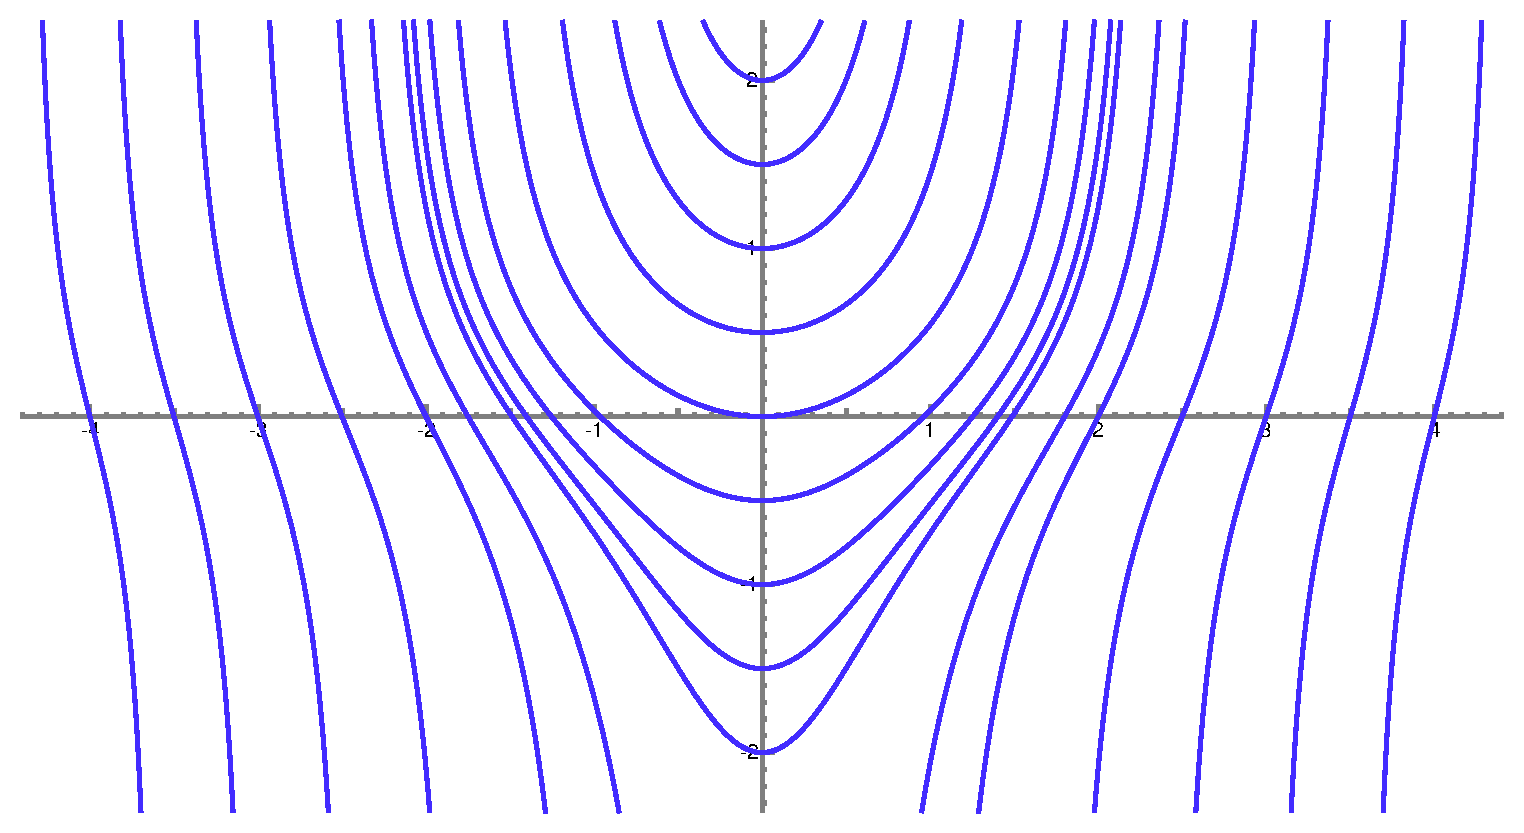
\includegraphics[width=0.8\textwidth]{fig_43856.pdf}
\label{fig:43856}
\caption{i grafici delle soluzioni dell'equazione differenziale~\eqref{eq:43856}.-}
\end{figure}

Osserviamo che la condizione~\eqref{eq:4856} equivale a richiedere che l'argomento
della tangente stia nell'intervallo $\enclose{-\frac \pi 2, \frac \pi 2}$.
In tal caso dovrà essere $c<\frac\pi 2$ e si osserva che se $c>-\frac \pi 2$
la soluzione $u(x)$ è definita su un intervallo aperto centrato in $x=0$ mentre
se $c \le -\frac \pi 2$ la soluzione è definita su una coppia di intervalli
simmetrici con ampiezza che tende a zero quando $c\to -\infty$.
Agli estremi di tali intervalli la soluzione ha degli asintoti verticali.

In questo caso possiamo osservare che la condizione~\eqref{eq:4856} può essere
trascurata, visto che la funzione $\tg$ è $\pi$-periodica e quindi
è possibile sommare a $c$ un multiplo intero di $\pi$ senza che la soluzione
venga modificata.
Nell'equazione~\eqref{eq:45876314} si potrebbe
quindi considerare la funzione $\tg$
definita su tutto il suo dominio osservando che in tal caso si può
supporre che sia $c\in \left(-\frac \pi 2, \frac \pi 2\right]$.
Invece di ottenere un singolo intervallo per ogni $c$ si ottengono così
tutti gli infiniti intervalli.
\end{example}

\begin{remark}
L'esempio precedente mette in evidenza il fatto che le soluzioni massimali possono essere definite
su intervalli arbitrariamente piccoli anche se l'equazione differenziale
non presenta singolarità. Diremo in questo caso che
la soluzione non è globale.
\end{remark}

\begin{example}
Si voglia risolvere l'equazione
\[
  u' = u^2.
\]
Si tratta di una equazione in forma normale, del primo ordine, autonoma.
In particolare è a variabili separabili
$u' = f(u(x))\cdot g(x)$
con $f(u)=u^2$ e $g(x)=1$.
Osserviamo innanzitutto che $u(x) = 0$ è soluzione in quanto $u'(x) = u^2(x) = 0$.
Se $u$ è una soluzione non identicamente nulla ci saranno dei punti in cui
$u(x)\neq 0$.
In un intorno di tali punti possiamo dividere ambo i membri dell'equazione per $u^2(x)$ ottenendo:
\[
  \frac{u'}{u^2} = 1.
\]
Integrando il lato sinistro tramite cambio di variabile $u=u(x)$, $du=u'(x)\, dx$ si ottiene:
\[
  \int \frac{u'(x)}{u^2(x)}\, dx = \Enclose{\int \frac{du}{u^2}}_{u=u(x)} = \Enclose{-\frac{1}{u}}_{u=u(x)}
  = -\frac{1}{u(x)}
\]
mentre integrando il lato destro si ha
\[
  \int 1 \, dx \ni x.
\]
Dunque su ogni intervallo in cui $u(x)\neq 0$ deve esistere una costante $c\in \RR$ tale che
\[
-\frac{1}{u(x)} = x + c
\]
ovvero, ponendo $x_0 = -c$
\begin{equation}\label{eq:5782196}
  u(x) = -\frac{1}{x+c} = \frac{1}{x_0-x}.
\end{equation}

In conclusione abbiamo trovato una soluzione costante $u(x)=0$ e una famiglia
di soluzioni definite sugli intervalli $(-\infty,x_0)$ e $(x_0,+\infty)$
rappresentante dall'equazione~\eqref{eq:5782196}.
Dovremmo ora chiederci
se è possibile che queste soluzioni vengano mescolate tra loro, ovvero
se una soluzione può valere zero in alcune zone e soddisfare~\eqref{eq:5782196}
in altre.

In questo caso la risposta è no.
Basta osservare che una funzione $u$ che soddisfa l'equazione~\eqref{eq:5782196}
può tendere a zero solamente quando $x\to +\infty$ o $x\to -\infty$.
Questo significa che se consideriamo una soluzione $u(x)$
definita su un intervallo $I$ e se in almeno un punto la soluzione è diversa da zero,
allora la soluzione è diversa da zero su tutto $I$ e
soddisfa l'equazione~\eqref{eq:5782196} in quanto la soluzione nulla e la
soluzione \eqref{eq:5782196} non sono tra loro compatibili (non possono essere
incollate con continuità).

Vedremo più avanti un risultato
(proposizione~\ref{prop:separazione_soluzioni})
che garantisce in ipotesi molto generali (che sono soddisfatte per questa
equazione) due diverse soluzioni non
possono mai incontrarsi.
\end{example}

\begin{exercise}
Fissato $p>1$ si risolva l'equazione differenziale
\[
  u' = u^p
\]
e si osservi che la soluzione presenta sempre un asintoto verticale
(dunque non c'è esistenza globale)-.++
\end{exercise}

\begin{example}[baffo di Peano]
Si determinino tutte le soluzioni del problema di Cauchy
\begin{equation}
\label{eq:94467}
\begin{cases}
  u'(x) = \sqrt[3]{u(x)}\\
  u(0)=0
\end{cases}
\end{equation}
\end{example}
%
\begin{figure}
\myurl{94467}{Il baffo di Peano formato dalle soluzioni del problema di Cauchy (\getrefnumber{eq:94467})}
\centering
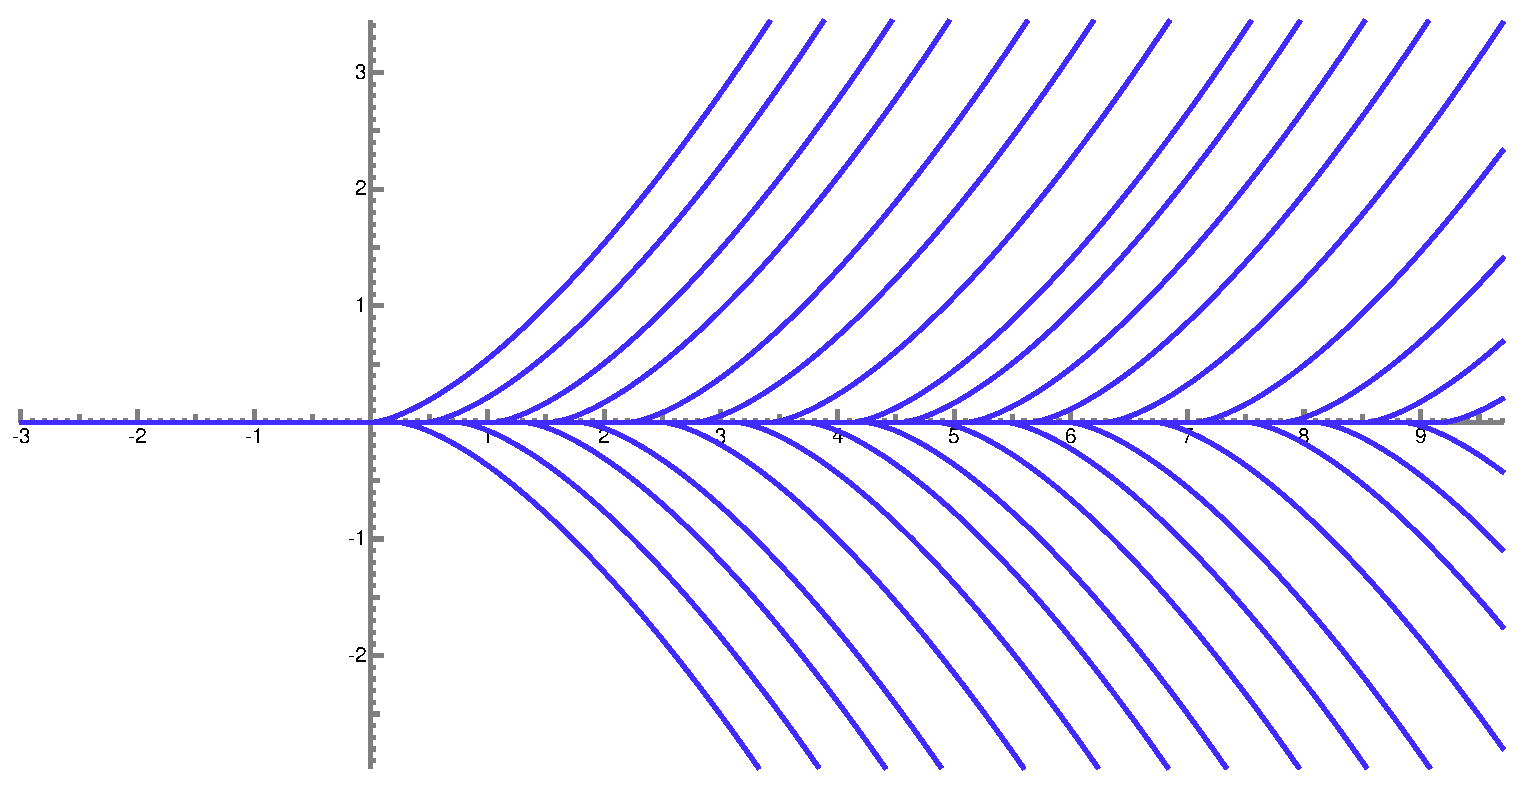
\includegraphics[width=0.9\textwidth]{fig_94467.pdf}
\label{fig:94467}
\caption{Il baffo di Peano formato dalle soluzioni del problema di Cauchy~\eqref{eq:94467}.}
\end{figure}
%
\begin{proof}[Svolgimento.]
Osserviamo che la funzione nulla $u(x)=0$ è soluzione dell'equazione
e soddisfa la condizione $u(0)=0$.
Ma a priori non possiamo escludere che ci siano altre soluzioni dell'equazione
che verifichino la stessa condizione (vedremo che la
proposizione~\ref{prop:separazione_soluzioni} non si applica in questo caso
particolare).

Nei punti in cui $u(x)\neq 0$ possiamo riscrivere l'equazione nella forma
\[
  \frac{u'(x)}{\sqrt[3]{u(x)}} = 1.
\]
Integrando il lato sinistro tramite il cambio di variabili $u=u(x)$,
$du = u'(x)\, dx$,
si ottiene
\[
  \int \frac{u'(x)}{\sqrt[3]{u(x)}}\, dx
  = \Enclose{\int \frac{du}{\sqrt[3]u}}_{u=u(x)}
  \ni \frac 3 2 \sqrt[3]{u^2(x)}.
\]
integrando anche il lato destro troviamo dunque
che su ogni intervallo su cui $u$ è definita e $u(x)\neq 0$
deve esistere una costante $c$ tale che
\[
  \frac 3 2 \sqrt[3]{u^2(x)} = x + c.
\]
Risolvendo in $u(x)$:
\begin{equation}\label{eq:476937568}
  u(x) = \pm \sqrt{\enclose{\frac 2 3 (x+c)}^3}.
\end{equation}
Osserviamo che la proprietà precedente
può essere soddisfatta solamente se $x\ge -c$ ma affinché
sia $u(x)\neq 0$ dobbiamo imporre $x>-c$.
Ma per $x\to -c^+$
si ha $u(x)\to 0$ e anche $u'(x) = \sqrt[3]{u(x)}\to 0$.
Significa che una soluzione definita su $x>c$ mediante
la~\eqref{eq:476937568} può essere estesa a tutto $\RR$
ponendo $u(x)=0$ per $x\le c$.
Affinché valga la condizione $u(0)=0$ sarà dunque sufficiente
imporre la restrizione $-c\ge 0$.

Il nostro problema ha dunque infinite soluzioni definite
su tutto $\RR$. Per la precisione, per ogni $c\ge 0$
(cambiamo segno alla costante trovata prima, in modo che risulti
positiva)
si hanno le soluzioni
\[
  u(x) = \begin{cases}
    0 & \text{per $x\le c$}\\
    \sqrt{\enclose{\frac 2 3 (x-c)}^3} & \text{per $x>c$}
  \end{cases}
\]
e
\[
  u(x) = \begin{cases}
    0 & \text{per $x\le c$}\\
    -\sqrt{\enclose{\frac 2 3 (x-c)}^3} & \text{per $x>c$}
  \end{cases}
\]
\end{proof}
\subsection{altri metodi risolutivi}

Nella sezione precedente abbiamo visto che le equazioni lineari del primo ordine
e le equazioni
a variabili separabili possono essere ricondotte al calcolo di una primitiva.
Nella sezione~\ref{sec:edo_lineari} verranno esposti i metodi risolutivi per le
equazioni lineari di ordine $n$ a coefficienti costanti.

Ci sono molti altri tipi di equazioni che possono essere ricondotti
alle equazioni lineari o alle equazioni a variabili separabili.
Non potremo dilungarci su questi metodi ma può essere utile,
come riferimento non esaustivo,
un elenco di alcune tipologie di equazioni per le quali esiste un metodo
risoluvtivo:

\begin{enumerate}
\item \emph{equazione del secondo ordine senza dipendenza da $u$}
\[
  F(x, u', u'') = 0
\]
si riconduce al primo ordine ponendo $v(x)=u'(x)$;
\item \emph{equazione del secondo ordine autonoma}
\[
  F(u, u', u'') = 0
\]
si riconduce al primo ordine
ponendo $v(u(x)) = u'(x)$;
\item \emph{equazione di Bernoulli}
\[
  u' = a(x) u + b(z) u^\alpha
\]
si riconduce ad una equazione lineare ponendo
$v(x) = u(x)^{1-\alpha}$;
\item \emph{equazione di Clairaut}
\[
  u = x u' + f(u');
\]
la derivata dell'equazione si fattorizza: un
fattore dà soluzioni della forma $u(x)=mx+q$ l'altro fattore diventa
una equazione algebrica facendo la sostituzione $u(x) = v(u'(x))$;
\item \emph{equazione di Riccati}
\[
  u' = u^2 + b(x) u + c(x).
\]
si ponga $u'(x) = -v'(x)/v(x)$ per ricondursi ad
una equazione lineare del secondo ordine in $v$;
\end{enumerate}

\begin{example}[equazione di Newton]
Un sistema fisico unidimensionale soggetto a forze che dipendono solamente
dalla posizione può essere descritto da un problema di Cauchy:
\[
\begin{cases}
  u''(x) = F(u(x)) \\
  u(x_0) = u_0 \\
  u'(x_0) = v_0
\end{cases}
\]
(ad esempio per il pendolo si ha $F(y) = -\sin y$).
La funzione $v$ definita da $v(u(x)) = u'(x)$ mette in relazione
la velocità con la posizione e descrive quindi il moto nel
cosiddetto \emph{spazio delle fasi}. Con tale sostituzione si
trova
\[
  u''(x) = v'(u(x)) u'(x) = v'(u(x)) v(u(x))
\]
che sostituita in $u'' = F(u)$ ci dà una equazione
differenziale del primo ordine per $v=v(u)$:
\[
 v' v  = F(u).
\]
Questa è una equazione del primo ordine a variabili separabili
che può essere interpretata come la legge di conservazione dell'energia,
infatti è equivalente a
\[
  \frac{d}{dx}\enclose{\frac 1 2 v^2 - \int F(u)} = 0
\]
dove $\frac 1 2 v^2$ si interpreta come energia cinetica e $-\int F$
come energia potenziale.
Integrando tra $x_0$ e $x$ e utilizzando le condizioni iniziali si ottiene,
con $u=u(x)$:
\[
  \frac 1 2 v^2(u) = \frac 1 2 v_0^2 + \int_{u_0}^{u} F(y)\, dy.
\]
Questa equazione descrive la traiettoria del sistema nel piano delle fasi $(u,v)$
e ci permette di ricavare $v$ in funzione di $u$:
\[
  v(u) = \pm\sqrt{v_0^2 + 2\int_{u_0}^u F(u)\, du}
\]
che significa:
\begin{equation}\label{eq:8844475}
  u'(x) = \pm \sqrt{v_0^2 + 2 \int_{u_0}^{u(x)} F(y)\, dy}.
\end{equation}
Questa è una equazione autonoma in $u$, quindi a variabili separabili:
\[
  \pm\frac{u'(x)}{\sqrt{v_0^2 - \int_{u_0}^{u(x)} F(y)\, dy}} = 1
\]
che può essere integrata tra $x_0$ e $x$ facendo il cambio di variabile $u=u(x)$
\[
  \pm\int_{u_0}^{u(x)} \frac{du}{\sqrt{v_0^2-\int_{u_0}^u F(y)\, dy}} = x-x_0.
\]
In questo modo abbiamo determinato la funzione inversa della soluzione $u(x)$.
\end{example}

\begin{example}[periodo del pendolo]
Sia $u(x)$
l'angolo di scostamento dalla verticale
al tempo $x$ di un pendolo semplice di lunghezza $\ell$.
Considerando la componente tangenziale della accelerazione di gravità
(il cui modulo è $g$)
l'equazione di Newton può essere scritta nella forma:
\[
  u''(x) = -\frac{g}{\ell} \sin u(x).
\]
Siamo quindi nel caso dell'esempio precedente dove $F(u) = -\frac{g}{\ell} \sin u$
e se al tempo $x=0$ lasciamo cadere da fermo il pendolo da un angolo $u_0$,
si avrà $v_0=0$. L'energia potenziale sarà data allora da
\[
-\frac{g}{\ell}\int_{u_0}^u \sin y\, dy = \frac{g}{\ell}\enclose{\cos u - \cos u_0}.
\]
L'equazione~\eqref{eq:8844475} diventa dunque
\[
  u'(x) = \pm \sqrt{2\frac{g}{\ell}(\cos u(x) - \cos u_0)}.
\]
Separando le variabili e integrando tra $0$ e $x$ si ottiene
\[
\sqrt{\frac \ell g}\int_0^x \frac{u'(t)\, dt}{\pm\sqrt{2\cos u(t)-2\cos u_0}}
= \int_0^x dt  = x.
\]
Cambiando variabile $u=u(x)$, $du = u'(x) dx$:
\begin{equation}\label{eq:4898944}
\sqrt{\frac \ell g}\int_0^{u(x)} \frac{du}{\pm\sqrt{2\cos u-2\cos u_0}} = x.
\end{equation}
La scelta del segno $\pm$ è arbitraria ma visto che $u$ è continua
anche $u'=-\sin u$ deve essere una funzione continua. Dunque il segno
$\pm$ può cambiare solo quando $u'=0$. Nel punto iniziale $x=0$ abbiamo
imposto $u'(0) = 0$ e dunque l'energia cinetica è nulla. Visto che l'energia
cinetica non può essere negativa significa che l'energia potenziale
non può aumentare e quindi inizialmente l'angolo $u(x)$ dovrà diminuire
(o almeno: non potrà aumentare). Dunque inizialmente il segno di $u'$ è negativo
e rimarrà negativo finché non si avrà nuovamente $u'(x)=0$.
L'integrale in~\eqref{eq:4898944} è un integrale improprio in quanto
la funzione integranda presenta un asintoto per $u\to u_0^-$ dobbiamo dunque
assicurarci che l'integrale sia finito. Sviluppando $\cos u$ nel punto $u=u_0$
si trova $\cos u = \cos u_0  - \sin u_0 \cdot (u-u_0) + o(u-u_0)$ da cui
\[
 \frac{1}{\sqrt{2 \cos u - 2 \cos u_0}}
 =\frac{1}{\sqrt{2\sin u_0\cdot (u_0-u) + o(u-u_0)}}
 \sim \frac{C}{\sqrt{u_0-u}}
\]
che è notoriamente una funzione integrabile per $u\to u_0^-$.

Vogliamo ora calcolare il tempo $x_1$ in cui il pendolo raggiunge per la prima
volta la verticale, cioè $u(x_1)=0$.
Ricordiamo che al tempo $x=0$ il pendolo parte da un angolo $u_0$
con velocità nulla. Nell'intervallo $x\in[0,x_1]$ si avrà $u'(x)<0$
(l'angolo diminuisce) dunque:
\[
-\sqrt{\frac{\ell}{g}}\int_{u_0}^{0} \frac{du}{\sqrt{2\cos u - 2\cos u_0}}
= x_1.
\]

Una volta raggiunta la verticale, per simmetria il pendolo tornerà a risalire
fino ad un angolo $-u_0$ mettendoci lo stesso tempo $x_1$. Poi tornerà a scendere
e risalire fino a tornare all'angolo $u_0$ mettendoci in totale un tempo
$T=4x_1$ che è quindi il periodo di oscillazione. Si ha dunque
\[
  \frac{T}{4} = \sqrt{\frac \ell g}\int_0^{u_0} \frac{du}{\sqrt{2\cos u - 2\cos u_0}}.
\]

Purtroppo l'integrale che abbiamo trovato non ha una primitiva
esprimibile mediante funzioni elementari (è un integrale ellittico).
Il nostro obiettivo è ora quello di farne uno sviluppo di Taylor
per $u_0\to 0$ che significa determinare
il periodo del pendolo per \myemph{piccole oscillazioni}.

Tramite formule di bisezione possiamo scrivere $\cos u = 1 - 2 \sin^2\frac u 2$
da cui
\[
 \sqrt{2\cos u - 2\cos u_0}
 = \sqrt{4\sin^2 \frac {u_0} 2 - 4 \sin^2 \frac{u}{2}}
 = 2\sin u_0 \sqrt{1-\enclose{\frac{\sin \frac u 2}{\sin \frac {u_0}2}}^2}
\]
dunque ponendo
\begin{equation}\label{eq:4847843}
 \sin t = \frac{\sin \frac u 2}{\sin \frac{u_0} 2}
\end{equation}
si ha
\[
  \sqrt{\frac \ell g} \cdot \frac T 4
  =  \int_0^{u_0} \frac{du}{2\sin \frac {u_0}2 \sqrt{1-\sin^2 t}}
  = \int_0^{u_0} \frac{du}{2\sin \frac{u_0}2 \cos t}
\]
ma per il cambio di variabile~\eqref{eq:4847843} si ha
\[
  \cos t \, dt = \frac{\cos \frac u 2 }{2 \sin \frac{u_0} 2}\, du
\]
ovvero
\[
 \frac{du}{2\sin \frac {u_0} 2 \cos t} = \frac{dt}{\cos \frac u 2}
 = \frac{dt}{\sqrt{1-\sin^2 t \sin^2\frac{u_0}{2}}}
\]
e quindi
\[
\sqrt{\frac g \ell} \cdot \frac{T}{4}
= \int_0^{\frac \pi 2} \frac{dt}{\cos \frac u 2}
= \int_0^{\frac \pi 2} \frac{dt}{\sqrt{1-\sin^2 \frac u 2}}
= \int_0^{\frac \pi 2} \frac{dt}{\sqrt{1-\sin^2 \frac{u_0}{2} \sin^2 t}}.
\]
Utilizzando ora la serie binomiale (teorema~\ref{th:serie_binomiale})
possiamo scrivere
\begin{align*}
\sqrt{\frac g \ell} \cdot\frac{T}{4}
&= \int_0^{\frac \pi 2} \sum_{k=0}^{+\infty}{-\frac 1 2 \choose k} \enclose{-\sin^2 t\sin^2 \frac{u_0}2}^{k}\, dt.\\
&= \int_0^{\frac \pi 2} \sum_{k=0}^{+\infty}\frac{(2k-1)!!}{(2k)!!} \enclose{\sin^2 t\sin^2 \frac{u_0}2}^{k}\, dt.
\end{align*}
in quanto si ha
\begin{align*}
  {-\frac 1 2 \choose k}
  &= \frac{\enclose{-\frac 1 2}\cdot \enclose{-\frac 3 2} \cdots \enclose{-\frac{2k-1} 2}}{k!}\\
  &= (-1)^k\frac{(2k-1)!!}{2^k \cdot k!} = (-1)^k \frac{(2k-1)!!}{(2k)!!}.
\end{align*}
Rispetto alla variabile $\sin^2 t$ dentro all'integrale abbiamo ora una serie di potenze
con coefficienti
\[
 a_k = \frac{(2k-1)!!}{(2k)!!} \enclose{\sin^2\frac{u_0} 2}^{k}
\]
e si verifica facilmente che
$  \frac{a_{k+1}}{a_k} \to \sin^2 \frac{u_0}{2}$
dunque la serie di potenze converge se
$ \sin^2 t \le \frac{1}{\sin^2 \frac{u_0}{2}}$
che significa semplicemente
$ \sin \frac u 2 < 1$.
Stiamo quindi facendo un integrale esteso all'intero raggio
di convergenza della serie. Sappiamo che la serie
converge totalmente e quindi uniformemente sugli intervalli
chiusi strettamente contenuti nel raggio di convergenza.
Visto che la serie è a termini positivi le somme parziali
convergono alla somma della serie e sono tutte inferiori
a tale somma.
Abbiamo già visto, inoltre, che la somma della serie
è integrabile con integrale finito.
Dunque possiamo applicare
il teorema di convergenza dominata (teorema~\ref{th:convergenza_dominata} con $f=g$)
per scambiare la serie con l'integrale:
\[
\sqrt{\frac g \ell} \cdot\frac{T}{4}
= \sum_{k=0}^{+\infty}\frac{(2k-1)!!}{(2k)!!} \enclose{\sin \frac{u_0}2}^{2k}
\int_0^{\frac \pi 2}  \enclose{\sin t}^{2k}\, dt
\]
l'integrale è ora sostanzialmente lo stesso $I_n$ che abbiamo calcolato nel teorema~\ref{th:wallis}:
\[
  \int_0^{\frac \pi 2} \enclose{\sin t}^{2k}\, dt
  = \frac 1 2 \int_0^{\pi} \enclose{\sin t}^{2k}\, dt
  = \frac{I_{2k}}{2}
  = \frac \pi 2 \cdot\frac{(2k-1)!!}{(2k)!!}
\]
da cui
\[
T
= 2\pi\sqrt{\frac \ell g}\sum_{k=0}^{+\infty} \enclose{\frac{(2k-1)!!}{(2k)!}}^2
\enclose{\sin \frac{u_0} 2}^{2k}.
\]

Possiamo allora cercare di scrivere i primi termini dello sviluppo di
Taylor di $T = T(u_0)$ per $u_0\to 0$ diciamo, per esempio, fino all'ordine 8
in $u_0$. Basterà considerare la somma dei termini della
serie per $k=0,1,2,3,4$ in quanto la somma dei termini per $k\ge 5$ mi darà
 un contributo dell'ordine di $O\enclose{\sin \frac {u_0} 2}^{10} = o(u_0^8)$. Dunque
 \begin{align*}
 \sqrt{\frac{g}{\ell}}\cdot \frac{T}{2\pi}
 &=
 1 + \enclose{\frac 1 2}^2 \sin^2 \frac{u_0} 2
 + \enclose{\frac{1\cdot 3}{2\cdot 4}}^2\enclose{\sin^2 \frac {u_0} 2}^2 \\
 &\quad + \enclose{\frac{1\cdot 3 \cdot 5}{2\cdot 4 \cdot 6}}^2
 \enclose{\sin^2 \frac {u_0} 2}^3 + \enclose{\frac{1\cdot 3\cdot 5 \cdot 7}{2\cdot 4\cdot 6\cdot 8}}^2
 \enclose{\sin^2 \frac {u_0} 2}^4 + o(u_0^8) \\
% \end{align*}
% \begin{align*}
 %
 &=
1 + \frac 1 4 \enclose{\frac{u_0^2}{4} - \frac{u_0^4}{2^4\cdot 3} + \frac{u_0^6}{2^5\cdot 3^2\cdot 5}
- \frac{u_0^8}{2^8\cdot 3^2\cdot 5\cdot 7}} \\
&\quad + \frac{3^2}{2^6}\enclose{\frac{u_0^2}{4} - \frac{u_0^4}{2^4\cdot 3}
+ \frac{u_0^6}{2^5\cdot 3^2\cdot 5}}^2\\
&\quad + \frac{5^2}{2^8}\enclose{\frac{u_0^2}{4} - \frac{u_0^4}{2^4\cdot 3}}^3
+ \frac{5^2\cdot 7^2}{2^{14}}
\frac {u_0^8} {2^8} + o(u_0^8)\\
%
%\end{align*}
%\begin{align*}
&=
1 + \frac{u_0^2}{2^4} - \frac{u_0^4}{2^6\cdot 3} + \frac{u_0^6}{2^7\cdot 3^2\cdot 5}
- \frac{u_0^8}{2^{10}\cdot 3^2\cdot 5\cdot 7} \\
&\quad + \frac{3^2}{2^6}\enclose{\frac{u_0^4}{2^4} - \frac{u_0^6}{2^5\cdot 3} + \frac{u_0^8}{2^8\cdot 3^2} + \frac{u_0^8}{2^6\cdot 3^2\cdot 5}}\\
&\quad + \frac{5^2}{2^8}\enclose{\frac{u_0^6}{2^6} - \frac{u_0^8}{2^8}}
+ \frac{5^2\cdot 7^2}{2^{22}}
u_0^8 + o(u_0^8)\\
%
% \end{align*}
% \begin{align*}
&= 1 + \frac{u_0^2}{2^4} + \frac{11}{2^{10}\cdot 3} u_0^4
 + \frac{173}{2^{14}\cdot 3^2\cdot 5} u_0^6
 + \frac{22931}{2^{22}\cdot 3^2\cdot 5\cdot 7} u_0^8
 + o(u_0^8).\\
\end{align*}

\end{example}

%%%%%%%%%%%%%%%%%%%%
%%%%%%%%%%%%%%%%%%%%
%%%%%%%%%%%%%%%%%%%%
\section[funzioni vettoriali e di più variabili]{alcuni risultati preparatori
sulle funzioni vettoriali e di più variabili}
%%%%%%%%%%%%%%%%%%%%
%%%%%%%%%%%%%%%%%%%%
%%%%%%%%%%%%%%%%%%%%

Ci sarà utile estendere la definizione delle classi di regolarità $C^k$ alle
funzioni vettoriali (cioè con codominio $\RR^n$) e di più variabili
(cioè con dominio $\RR^m$).

Se $\Omega\subset \RR^m$ è un insieme aperto e $f\colon \Omega \to \RR$
è una funzione, vogliamo definire le \emph{derivate parziali} di $f$.
Se $\vec x \in \Omega$ si ha $\vec x = (x_1,\dots, x_m)$ e quindi
$f(\vec x) = f(x_1,\dots, x_m)$. Se facciamo variare una sola componente
$x_j$ mantenendo fisse tutte le altre componenti, otteniamo una funzione
di una variabile $x_j \mapsto g(x_j) = f(x_1,\dots, x_j, \dots, x_m)$.
Definiamo dunque la \emph{derivata parziale}
\mynote{derivata parziale}
\index{derivata!parziale}
di $f$ rispetto alla variabile $x_j$ come la derivata della funzione $g(x_j)$.
Denotiamo tale derivata con il simbolo:
\[
  \frac{\partial f}{\partial x_j}.
\]
Le derivate parziali si calcolano dunque come le usuali derivate per le
funzioni di una variabile, solamente bisogna considerare costanti tutte
le variabili tranne quella coinvolta nella derivazione.
Ad esempio se $f(x,v) = -\sin(x) - v$
(come nell'esempio fatto nell'introduzione) si ha
\begin{align*}
  \frac{\partial f}{\partial x} &= -\cos(x)\\
  \frac{\partial f}{\partial v} &= -1.
\end{align*}

Se $\vec f\colon \Omega \subset \RR^m \to \RR^n$ è una funzione di più
variabili a valori vettoriali potremo scrivere $\vec f = (f_1, \dots, f_n)$
e considerare le derivate parziali di ogni componente:
\[
  \frac{\partial \vec f}{\partial x_j}
  = \enclose{\frac{\partial f_1}{\partial x_j}, \dots, \frac{\partial f_n}{x_j}}.
\]

\begin{definition}
Sia $\Omega\subset \RR^m$ un aperto. Denoteremo con $C^0(\Omega,\RR^n)$
lo spazio vettoriale di tutte le funzioni
continue $f\colon \Omega \to \RR^n$.

Denotiamo con $C^1(\Omega,\RR^n)$ lo spazio vettoriale
delle funzioni in $C^0(\Omega,\RR^n)$ tali che ognuna delle loro derivate
parziali $\frac{\partial f}{\partial x_j}$ esiste in ogni punto di $\Omega$ ed
è a sua volta una funzione continua (cioè in $C^0(\Omega,\RR^n)$).
Ricorsivamente si definisce $C^k(\Omega,\RR^n)$ per $k>1$,
come lo spazio delle funzioni $\Omega\to\RR^n$ tali che tutte le loro derivate
parziali stanno in $C^{k-1}(\Omega,\RR^n)$.

Quando lo spazio di arrivo non è indicato si sottointende sempre $\RR$, quindi
$C^k(\Omega) = C^k(\Omega,\RR)$.
\end{definition}

\begin{theorem}[stabilità delle funzioni regolari]
Sia $\Omega \subset \RR^n$ un aperto.
Se $f,g\in C^k(\Omega)$ allora anche $f+g$, $f-g$, $f\cdot g$ e $\frac{f}{g}$
(dove è definita) sono di classe $C^k$. Se $f\in C^k(\Omega)$ e $g\in C^k(\RR)$
allora $g\circ f \in C^k(\Omega)$.
\end{theorem}
%
\begin{proof}
Il fatto che la composizione di funzioni continue sia una funzione continua
è vero in generale in qualunque spazio metrico.
Infatti se $f\colon X\to Y$ e $g\colon Y \to Z$ e se $x_k\to x$ in $X$
allora $f(x_k) \to f(x)$ in $Y$ (per la continuità di $f$)
e quindi $g(f(x_k)) \to g(f(x))$ in $Z$ (per la continuità di $g$).
Dunque $(f \circ g)(x_k) \to (f\circ g)(x)$ e $f\circ g\colon X\to Z$ è continua.

Possiamo dunque osservare che le funzioni di due variabili $s(x,y) = x+y$,
$m(x,y)=xy$ sono funzioni continue da $\RR^2\to \RR$. Questo garantisce
che la somma e il prodotto di funzioni continue siano funzioni continue.
Anche l'opposto e il reciproco di funzioni continue sono funzioni continue
in quanto le funzioni $o(x)=-x$ e $r(x)=1/x$ sono continue.
Ne consegue che anche la differenza e il rapporto di funzioni continue sono
funzioni continue.

Veniamo ora alle derivate parziali.
Per le regole di derivazione delle funzioni di una variabile sappiamo che
somma, prodotto, differenza, rapporto (ove definito) e composizione
di funzioni derivabili sono
a loro volta funzioni derivabili e la derivata si esprime sempre mediante
somma, prodotto, differenza e rapporto delle funzioni coinvolte e delle loro
derivate. Dunque quello che si ottiene combinando tra loro funzioni
di classe $C^k$ è una funzione continua le cui derivate parziali esistono e
sono di classe $C^{k-1}$, dunque è una funzione di classe $C^k$.
\end{proof}

\begin{definition}
Sia $\vec f\colon [a,b]\to \RR^m$, $\vec f(x) = (f_1(x), \dots, f_m(x))$.
Diremo che $\vec f$ è integrabile su $[a,b]$ se ogni
$f_k\colon[a,b]\to \RR$ è integrabile su $[a,b]$ e in tal caso porremo:
\[
  \int_a^b \vec f(x)\, dx
  = \enclose{\int_a^b f_1(x)\, dx, \dots, \int_a^b f_m(x)\, dx}
  \in \RR^m
\]
cosicché per ogni $k=1,\dots, m$ si ha:
\[
  \enclose{\int_a^b \vec f(x)\, dx}_k = \int_a^b f_k(x)\, dx.
\]
Come al solito si pone inoltre $\int_b^a \vec f = - \int_a^b \vec f$.
\end{definition}

\begin{theorem}\label{teo:tipo_jensen}
\mymark{*}
Sia $\vec f\colon [a,b]\to \RR^m$ integrabile. Allora si ha
\[
  \abs{\int_a^b \vec f(x)\, dx} \le \int_a^b \abs{\vec f(x)}\, dx.
\]
\end{theorem}
%
\begin{proof}
Posto
\[
 \vec v = \int_a^b \vec f(x)\, dx
\]
si ha, usando la linearità dell'integrale
e sfruttando la disuguaglianza di Cauchy-Schwarz
\begin{align*}
  \abs{\vec v}^2
  &= \vec v \cdot \vec v
   = \sum_{k=1}^n v_k \int_a^b f_k(x)\, dx
   = \int_a^b \sum_{k=1}^m v_k f_k(x)\, dx \\
  &= \int_a^b \enclose{\vec v, \vec f(x)}\, dx
  \le \int_a^b \abs{\vec v}\cdot \abs{\vec f(x)}\, dx
  = \abs{\vec v} \int_a^b \abs{\vec f(x)}\, dx.
\end{align*}
Se $\abs{\vec v}\neq 0$ possiamo dividere ambo i membri per $\abs{\vec v}$ e
ottenere la disuguaglianza cercata.
Altrimenti se $\abs{\vec v}=0$ la disuguaglianza è certamente soddisfatta in
quanto il lato destro non può essere negativo.
\end{proof}


%%%%%
%%%%%
%%%%%
%%%%%
\section{Il problema di Cauchy}
%%%%%
%%%%%
%%%%%
%%%%%

Il problema di Cauchy
per i sistemi del primo ordine
consiste nel
trovare una soluzione di un sistema di $n$ equazioni differenziali ordinarie del primo ordine in $n$ incognite
con un dato iniziale fissato. Cioè dato $x_0\in \RR$,
e $\vec y_0 \in \RR^n$ si cerca un intervallo $I\subset \RR$ con $x_0\in I$ e una funzione $\vec u \colon I\to \RR^n$
che sia derivabile e che soddisfi:
\begin{equation}\label{eq:problema_cauchy}
\begin{cases}
 \vec u'(x) = \vec f(x, \vec u(x)), \qquad \forall x\in I\\
 \vec u(x_0) = \vec y_0.
\end{cases}
\end{equation}

\begin{definition}[Cauchy-Lipschitz]
\label{def:cauchy_lipschitz}
Diremo che una funzione $\vec f\colon \Omega\subset \RR\times \RR^n \to \RR^m$
soddisfa la \myemph{proprietà di Cauchy-Lipschitz} se $f$ è continua e se
per ogni $(x_0,\vec y_0)\in \Omega$ esiste un intorno $U$ di $(x_0,\vec y_0)$
ed esiste $L\ge 0$
tale che se $(x,\vec y_1)\in U$ e $(x,\vec y_2)\in U$ si ha
\[
  \abs{\vec f(x,\vec y_1)- \vec f(x,\vec y_2)} \le L \abs{\vec y_1- \vec y_2}
\]
A parole potremmo dire: $\vec f(x,\vec y)$ è localmente lipschitziana rispetto
a $\vec y$ uniformemente
rispetto a $x$.
\end{definition}

\begin{theorem}[Cauchy-Lipschitz, esistenza e unicità locale]
\label{th:cauchy_lipschitz}
\mymargin{esistenza e unicità locale per i sistemi del primo ordine}
\mymark{***}
Sia $\Omega$ un aperto di $\RR\times \RR^n$ e sia $\vec f\colon \Omega \to \RR^n$,
una funzione con la proprietà di Cauchy-Lipschitz
(definizione~\ref{def:cauchy_lipschitz}).

Allora dato $(x_0,\vec y_0)\in \Omega$
esiste $\delta>0$
tale che preso qualunque intervallo $I\subset [x_0-\delta,x_0+\delta]$
con $x_0\in I$
esiste una unica funzione $\vec u\colon I \to \RR^n$
tale che $(x,\vec u(x))\in \Omega$ per ogni $x\in I$
che soddisfa il problema di Cauchy~\eqref{eq:problema_cauchy}.
\end{theorem}
%
%
\begin{proof}
\mymark{***}
L'idea della dimostrazione è che integrando ambo i lati dell'equazione
$\vec u' = f(x,\vec u)$ e tenendo conto della condizione iniziale, si
ottiene una equazione del tipo $\vec u = T(\vec u)$ dove $T$ è un operatore
sullo spazio delle funzioni continue.
Scegliendo $\delta$ abbastanza piccolo si riuscirà a mostrare che le funzioni
definite su un intervallo di raggio $\delta$ intorno a $x_0$ risultano
essere uno spazio invariante per $T$ e, eventualmente rimpicciolendo ulteriormente
$\delta$ si riuscità poi a dimostrare che $T$ è una contrazione e quindi
l'esistenza e unicità della soluzione si ottiene
dal teorema del punto fisso di Banach-Caccioppoli.

Il primo passo è quello di trasformare il problema differenziale in un problema
integrale.
Se $\vec u$ è una funzione derivabile soluzione di \eqref{eq:problema_cauchy}
allora è chiaro che $\vec u'(x) = \vec f(x,\vec u(x))$ è continua in quanto
composizione di funzioni continue e dunque $\vec u$ è di classe $C^1$.
Possiamo dunque integrare tra $x_0$ e $x$ i due lati dell'equazione
differenziale per ottenere:
\[
  \vec u(x) - \vec u(x_0) = \int_{x_0}^x \vec f(s,\vec u(s))\, ds
\]
e dunque se $\vec u$ risolve il problema di Cauchy allora $\vec u$ soddisfa anche
la seguente equazione integrale:
\begin{equation}\label{eq:cauchy_integrale}
  \vec u(x) = \vec y_0 + \int_{x_0}^x \vec f(s,\vec u(s))\, ds.
\end{equation}
Viceversa se $\vec u$ è continua e soddisfa \eqref{eq:cauchy_integrale}
allora si ha ovviamente
$\vec u(x_0) = \vec y_0$ e,
passando alle derivate (grazie al teorema di Torricelli-Barrow~\ref{th:torricelli-barrow}),
si scopre che $\vec u$ è
derivabile e soddisfa l'equazione differenziale $\vec u'(x) = \vec f(x,\vec u(x))$.
Dunque trovare una soluzione $C^1$ del problema di Cauchy~\eqref{eq:problema_cauchy}
è equivalente a trovare una soluzione $C^0$ del problema integrale~\eqref{eq:cauchy_integrale}.
Ci dedicheremo dunque a questo secondo problema.

Fissato $(x_0, \vec y_0)$ denotiamo con
\[
  C_{\alpha,\beta} =
  \ENCLOSE{(x,\vec y)\in \RR\times\RR^n\colon \abs{x-x_0}\le \alpha, \abs{\vec y -\vec y_0}\le \beta}
\]
il cilindro centrato in $(x_0, \vec y_0)$ con asse parallelo all'asse delle $x$,
di altezza $2\alpha$ e raggio $\beta$.
Consideriamo l'intorno $U$ di $(x_0,\vec y_0)$ in cui, per ipotesi,
la funzione $\vec f$ è $L$-lipschitziana uniformemente rispetto ad $x$.
L'intorno $U$ conterra certamente un cilindro $C_{\alpha,\beta}$ per un qualche $\alpha>0$ e $\beta>0$
sufficientemente piccoli.
Il cilindro $C_{\alpha,\beta}$ è chiuso e limitato in $\Omega$ e dunque $\vec f$,
essendo continua, è limitata su $C_{\alpha,\beta}$ per il teorema di Weierstrass.
Sia $M>0$ tale che $\abs{\vec f(x,\vec y)}\le M$ per ogni
$(x,\vec y) \in C_{\alpha,\beta}$ e definiamo
\begin{equation}\label{eq:395109}
 \delta = \min\ENCLOSE{\alpha, \frac{\beta}{M}, \frac{1}{2L}}.
\end{equation}
Il perché $\delta$ venga definito in questo modo si capirà nel prosieguo della dimostrazione.
Consideriamo un qualunque intervallo $I\subset [x_0-\delta,x_0+\delta]$ e
definitamo lo spazio di funzioni
\[
X=\{\vec u\in C^0(I,\RR^n)\colon \Abs{\vec u-\vec y_0}_\infty
\le \beta \}.
\]
Sappiamo che $C^0(I,\RR^n)$ è uno spazio metrico completo e $X$ è chiuso quindi
anch'esso è completo. Possiamo allora considerare l'operatore
$T\colon X \to C^0(I, \RR^n)$ definito da:
\[
  T(\vec u)(x) = \vec y_0 + \int_{x_0}^x \vec f(s, \vec u(s))\, ds.
\]
Vogliamo innanzitutto verificare che $X$ è invariante,
cioè che $T(X)\subset X$.
Se $\vec u \in X$ e se $x\in I$ si ha
$(x,\vec u(x)) \in C_{\delta,\beta} \subset C_{\alpha,\beta}$
e dunque (usando anche~\eqref{eq:395109} e il teorema~\ref{teo:tipo_jensen})
\[
  \abs{\vec T(u)(x)-\vec y_0}
  = \abs{\int_{x_0}^x \vec f(s,\vec u(s))\, ds}
  \le \int_{x_0}^x M\, ds = \abs{x-x_0} M \le \delta M
  \le \beta.
\]
Dunque $\Abs{T(\vec u)-\vec y_0}\le \beta$ e $T(\vec u)\in X$.
Abbiamo dunque che $T\colon X \to X$. Verifichiamo ora che $T$ è una contrazione.
Si ha:
\begin{align*}
  \abs{T(\vec u_1)(x)-T(\vec u_2)(x)}
   &\le \abs{\int_{x_0}^x\abs{\vec f(s,\vec u_1(s))-\vec f(s,\vec u_2(s))}\, ds}\\
   &\le \abs{\int_{x_0}^x L\abs{\vec u_1(s)-\vec u_2(s)}\, ds}\\
   &\le L \abs{x-x_0}\Abs{\vec u_1 - \vec u_2}_\infty
   \le L \delta \Abs{\vec u_1 - \vec u_2}_\infty
\end{align*}
ovvero, facendo l'estremo superiore al variare di $x\in I$:
\[
 \Abs{T(\vec u_1)-T(\vec u_2)}_\infty
 \le L \delta \Abs{\vec u_1 - \vec u_2}_\infty
 \le \frac{1}{2}\Abs{\vec u_1- \vec u_2}.
\]
Dunque $T\colon X \to X$ è una contrazione su uno spazio metrico completo.
Per il teorema di punto fisso di Banach-Caccioppoli
\ref{th:banach-caccioppoli}
sappiamo quindi che esiste una unica funzione
$\vec u \in X$ ovvero $\vec u \colon I \to \RR^n$ che soddisfa
$T(\vec u)=\vec u$ ovvero~\eqref{eq:cauchy_integrale}
ovvero~\eqref{eq:problema_cauchy}.
\end{proof}

La condizione di Cauchy-Lipschitz può sembrare piuttosto complicata
da verificare. Una condizione molto più semplice  è che la funzione $\vec f$
sia di classe $C^1$. La seguente proposizione ci dice che tale
condizione è sufficiente per applicare il teorema di Cauchy-Lipschitz.

\begin{proposition}
\mymark{***}
Sia $\Omega \subset \RR\times \RR^n$ un insieme aperto.
Se $\vec f\in C^1(\Omega,\RR^m)$ allora $f$ soddisfa la condizione
di Cauchy-Lipschitz \ref{def:cauchy_lipschitz}.
\end{proposition}
%
\begin{proof}
\mymark{***}
Se prendiamo un qualunque cubo\footnote{%
Un cubo di lato $2L$ centrato nel punto $\vec p = (p_1,\dots,p_n)$
in $\RR^n$ di $\RR^n$ è l'insieme dato dal prodotto cartesiano
$K=[p_1-L,p_1+K]\times \dots \times [p_n-L,p_n+L]$}
chiuso $K \subset \Omega \subset \RR\times \RR^n$
centrato in $(x_0,\vec y_0)$, posto $\vec f = (f_1, \dots, f_m)$
sappiamo che ogni derivata parziale
$\partial f_k / \partial y_j$ è continua ed è quindi limitata
(per il teorema di Weierstrass) su $K$. Sia $L_{k,j}$ il massimo di $\abs{\partial f_k / \partial y_j}$ su $K$ e sia
$L$ il massimo degli $L_{k,j}$ per $k=1,\dots m$ e $j=1\dots,n$.
Allora presi $\vec y, \vec z \in \RR^n$ con $(x,\vec y),(x,\vec z)\in K$ si può scomporre l'incremento vettoriale $\vec z - \vec y$ lungo le $n$ direzioni coordinate e applicare il teorema di Lagrange lungo ogni direzione.
Per ogni $k = 1,\dots, m$ si ha quindi:
\begin{align*}
\MoveEqLeft
\abs{f_k(x,\vec z)-f_k(x,\vec y)}\\
&\le \sum_{j=1}^n \abs{f_k(x,z_1, \dots, z_j, y_{j+1}, \dots, y_n) - f_k(x,z_1, \dots, z_{j-1}, y_j, \dots, y_n)}\\
&\le \sum_{j=1}^n L_j \abs{z_j-y_j}
\le \sum_{j=1}^n L_j \abs{z-y}
\le n L \abs{z-y}
\end{align*}
da cui
\begin{align*}
  \abs{\vec f(x,\vec z) - \vec f(x,\vec y)}
  &= \sqrt{\sum_{k=1}^m \abs{f_k(x,\vec z) - f_k(x,\vec y)}^2} \\
  &\le \sqrt{\sum_{k=1}^m n^2 L^2 \abs{z-y}^2} \\
  &\le n\sqrt{m} L \abs{z-y}.
\end{align*}
Abbiamo quindi mostrato che per ogni $(x_0,\vec y_0)\in \Omega$ esiste un intorno del punto $(x_0,\vec y_0)$ in cui la funzione $\vec f$ soddisfa la condizione di Cauchy-Lipschitz.
\end{proof}

\begin{comment}

\begin{theorem}[maggiore regolarità delle soluzioni]
Sia $\vec u(x)$ una soluzione del sistema di
equazioni differenziali:
\[
  \vec u'(x) = \vec f(x, \vec u(x)).
\]
Se $\vec f\colon \Omega\subset \RR\times\RR^n \to\RR^n$ è una funzione di classe $C^k$, con $k\in \NN$ allora la soluzione $\vec u(x)$ è di classe $C^{k+1}$.
In particolare se $\vec f \in C^\infty$ anche $u\in C^\infty$.
\end{theorem}
%
\begin{proof}
Se $\vec u$ soddisfa l'equazione differenziale significa quanto meno che $\vec u$ è derivabile. Dunque è continua e derivabile e la derivata è
\[
  \vec u'(x) = \vec f(x,\vec u(x)).
\]
Ma il lato destro è composizione di funzioni continue (in quanto al minimo $\vec f \in C^0$ e $u\in C^0$) dunque la derivata di $u$ è di classe $C^0$. Significa che come minimo $\vec u$ è di classe $C^1$. Se ora $k\ge 1$ possiamo ripetere il procedimento e osservare che $\vec u'(x)$ è uguale ad una composizione di funzioni $C^1$, dunque è di classe $C^1$. Ma allora $\vec u$ è di classe $C^2$.
Il procedimento può essere dunque iterato fino ad arrivare a dedurre che $\vec u$ è di classe $C^k$. A quel punto la funzione $f(x,\vec u(x))$ è di classe $C^k$ e quindi $\vec u'$ è di classe $C^k$ e $\vec u$ è di classe $C^{k+1}$. Non si può iterare ulteriormente perché ora componendo una funzione $C^k$ con una funzione $C^{k+1}$ quello che ottengo è di nuovo $C^k$.

Dire che $f\in C^\infty$ significa che $f\in C^k$ per ogni $k$. Dunque $\vec u$ risulta essere di classe $C^{k+1}$ per ogni $k$: dunque diremo che $\vec u$ è di classe $C^\infty$.
\end{proof}
\end{comment}

Il teorema di Cauchy-Lipschitz garantisce l'esistenza di una soluzione
definita in un
piccolo intervallo $[x_0-\delta_0, x_0+\delta_0]$ intorno al punto iniziale $x_0$.
Se scegliamo $x_1 = x_0+\delta_0$ possiamo applicare nuovamente lo stesso
teorema per trovare una soluzione definita nell'intervallo
$[x_1-\delta_1, x_1+\delta_1]$
che coincida con la precedente soluzione nel punto $x_1$.
Le due soluzioni coincidono sull'intersezione dei due intervalli (grazie
all'unicità della soluzione su ogni sotto-intervallo) e quindi possono
essere incollate per ottenere una soluzione definita sull'unione dei due intervalli.
Questo procedimento può essere ripetuto infinite volte ma gli intervalli
potrebbero diventare sempre più piccoli, quindi non c'è garanzia di ottenere una
soluzione definita su intervalli arbitrariamente grandi.
Nel seguito cercheremo di capire quanto grande può essere l'intervallo
\emph{massimale} su cui si riesce ad estendere la soluzione.

\begin{definition}[soluzione/intervallo massimale]
Sia $I\subset \RR$ un intervallo non vuoto e sia $\vec u \colon I \to \RR^n$
una soluzione di una equazione differenziale.

Se $J\supset I$, $J \neq I$ è un intervallo, se $\vec v\colon J \to \RR^n$
risolve la stessa equazione differenziale
e se $\vec v(x)=\vec u(x)$ per ogni $x\in I$,
diremo che $\vec v$ è una \myemph{estensione della soluzione} $u(x)$.

Se la soluzione $\vec u$ non ammette estensioni, diremo che $\vec u$ è una
soluzione definita su un intervallo massimale o, più semplicemente, diremo
che $\vec u$ è una \myemph{soluzione massimale}.
\end{definition}

\begin{proposition}[caratterizzazione delle soluzioni massimali]
\label{prop:edo_massimale}
Supponiamo che $\vec f\colon \Omega\subset \RR\times\RR^n\to\RR^n$
soddisfi la condizione di Cauchy-Lipschitz \ref{def:cauchy_lipschitz}.
Allora una soluzione $\vec u$ dell'equazione
\begin{equation}\label{eq:edo_normale_ordine_uno}
  \vec u'(x) = \vec f(x, \vec u(x))
\end{equation}
è definita su un intervallo massimale $I$ se e solo se
$I$ è aperto e per ogni $K$ compatto $K\subset \Omega$
e per ogni $x_0 \in I$ esistono $x_1,x_2\in I$, $x_1 < x_0 < x_2$ tali che $\vec u(x_1)\not \in K$ e $\vec u(x_2) \not \in K$.
Significa cioè che il grafico di $\vec u$ cioè la curva $(x,\vec u(x))$ esce da qualunque compatto  $K\subset \Omega$ sia facendo crescere $x$ verso destra che facendo calare $x$ verso sinistra.
Intuitivamente il grafico della soluzione massimale tende ad arrivare ai limiti di $\Omega$.
\end{proposition}
%
\begin{proof}
\emph{Prima implicazione}.
Supponiamo che $\vec u\colon I \to \RR^n$ sia una soluzione di~\eqref{eq:edo_normale_ordine_uno} definita su un intervallo massimale $I$. Dovrà essere $(x,\vec u(x))\in \Omega$ per ogni $x\in I$.

Mostriamo innanzitutto
che $I$ è un intervallo aperto a destra: se non lo fosse si avrebbe che $x_0=\sup I \in I$. Allora $(x_0,\vec u(x_0))\in \Omega$ e per il teorema di esistenza e unicità locale
potremmo trovare un intorno $J$ di $x_0$ e una funzione
$\vec v\colon J\to \RR^n$ che risolve~\eqref{eq:edo_normale_ordine_uno}
con $\vec v(x_0)=\vec u(x_0)$.
Per l'unicità delle soluzioni $\vec u$ e $\vec v$ devono coincidere su $I\cap J$ e dunque facendo l'unione dei due grafici ottengo una estensione di $\vec u$ a tutto l'intervallo
$I\cup J$ che è strettamente più grande di $I$. Dunque $\vec u$ non poteva essere una soluzione massimale.

Mostriamo ora che la curva $(x,\vec u(x))$ esce da ogni compatto $K\subset \Omega$ sia da destra che da sinistra. Supponiamo per assurdo che esista un compatto $K$ tale che $(x,\vec u(x))\in K$ per ogni $x\in I$.
Il grafico $(x,\vec u(x))$ è limitato per $x\in I$ dunque certamente $I$ deve essere limitato. Inoltre abbiamo visto che $I$ è aperto e quindi $I=(a,b)$ con $a,b\in \RR$, $a<b$.

Allora per ogni $x\in I=(a,b)$ si ha
\[
  \abs{\vec u'(x)} = \abs{\vec f(x, \vec u(x))}
   \le \sup_K \abs{\vec f}.
\]
Visto che $\vec f$ è continua (in quanto soddisfa le ipotesi del teorema di esistenza e unicità) la funzione $\abs{\vec f}$ ha massimo su $K$ per il teorema di Weierstrass e quindi esiste $M\ge 0$ tale che $\abs{\vec u'(x)} \le M$ per ogni $x\in (a,b)$. Significa che ogni componente di $\vec u$ è $M$-lipschitziana, in particolare
ogni componente è uniformemente continua (teorema~\ref{th:lipschitz_uniformemente_continua}).
Dunque la funzione $\vec u$ può essere estesa con continuità
(teorema~\ref{th:estensione_uniformemente_continua})
ad una funzione $\vec v \colon [a,b] \to \RR^n$ definita anche agli estremi dell'intervallo.
Visto che $(x,\vec u(x)) \in K$ per ogni $x\in(a,b)$ e visto che
$\vec v(b) = \lim_{x\to b^-}\vec u(x)$ essendo $K$ chiuso possiamo affermare che
$(b,\vec v(b)) \in K$.
Lo stesso vale per $x\to a^+$ dunque $(a,\vec v(a))\in K$
e dunque $(x,\vec v(x))\in K \subset \Omega$ per ogni $x\in [a,b]$.
Vogliamo ora verificare che $\vec v$ è soluzione dell'equazione differenziale~\eqref{eq:edo_normale_ordine_uno}.
Chiaramente $\vec v$ soddisfa l'equazione per ogni $x\in (a,b)$
in quanto su $(a,b)$ coincide con $\vec u$ che è soluzione.
Consideriamo l'estremo $b$.
Visto che $\vec v$ è continua in $b$ e $\vec f$ è continua in $(b,\vec v(b))$ si ha
\[
  \lim_{x\to b^-} \vec v'(x)
  = \lim_{x\to b^-} \vec f(x,\vec  v(x))
  = \vec f(b,\vec v(b)) \in \RR^n
\]
Sappiamo però che se il limite della derivata di una funzione continua esiste ed è finito, allora la funzione è derivabile nel punto limite e la derivata è continua in quel punto
(proposizione~\ref{prop:4384774}).
Dunque $\vec v$ è derivabile in $b$ e anche in quel punto soddisfa l'equazione differenziale. Lo stesso vale nel punto $a$. Dunque siamo riusciti a trovare una estensione $\vec v$ di $\vec u$ contraddicendo l'ipotesi che $\vec u$ fosse una soluzione massimale.

\emph{Seconda implicazione}. Supponiamo ora $\vec u\colon I\to \RR^n$ sia una soluzione dell'equazione differenziale~\eqref{eq:edo_normale_ordine_uno} definita su un intervallo $I$ e tale che la curva $(x,\vec u(x))$ esca da ogni compatto $K$ al variare di $x\in I$. Vogliamo dimostrare che $\vec u$ è soluzione massimale. Innanzitutto $I$ non può essere compatto, altrimenti anche $K=\ENCLOSE{(x,\vec u(x))\colon x \in I}$ sarebbe un compatto di $\Omega$ e ovviamente la curva non esce da $K$.
Sia $a=\inf I$ e $b=\sup I$. Siccome $I$ non è chiuso esso non contiene uno dei due estremi: supponiamo sia $b$. Allora se $\vec u$ fosse estendibile a destra esisterebbe una estensione continua $\vec v\colon (a,b]\to \RR^n$ che coincide con $\vec u$ su $(a,b)$ e che è continua nel punto $x=b$ e che soddisfa l'equazione differenziale quindi, in particolare, $(b,\vec v(b))\in \Omega$.
Ma allora scelto $x_0 \in (a,b)$
prendiamo $K=\ENCLOSE{(x,\vec v(x))\colon x\in [x_0,b]}$. Visto che $\vec v\colon[x_0,b]\to \RR^n$ è continua è facile verificare che $K$ è chiuso è limitato, $K\subset \Omega$. Ma ovviamente $(x,\vec v(x))\in K$ per ogni $x\ge x_0$, contro le ipotesi.
\end{proof}

\begin{proposition}[separazione delle soluzioni]
\label{prop:separazione_soluzioni}
Se $\vec f\colon \Omega\subset \RR \times \RR^n\to \RR^n$ soddisfa
la condizione di Cauchy-Lipschitz
e se $\vec u\colon I \to \RR^n$ e $\vec v\colon J\to\RR^n$ sono due soluzioni
dell'equazione differenziale
$\vec u'(x) = \vec f(x,\vec u(x))$
definite su due intervalli $I,J \subset \RR$  e se esiste $x_0\in I\cap J$ tale che $\vec u(x_0) = \vec v(x_0)$ allora $\vec u(x) = \vec v(x)$ per ogni $x\in I\cap J$.
Detto in altri termini: nelle ipotesi del teorema di esistenza e unicità i grafici di due soluzioni diverse definite in un intervallo non possono toccarsi.
\end{proposition}
%
\begin{proof}
Sia $x_0 \in I\cap J$ un punto in cui $\vec u(x_0) = \vec v(x_0)$
e supponiamo per assurdo che esista $x_2 \in I\cap J$ tale che $\vec u(x_2)\neq \vec v(x_2)$. In tal caso possiamo considerare il punto
\[
   x_1 = \sup \ENCLOSE{x \in [x_0,x_2] \colon \vec u(x) = \vec v(x)}.
\]
Su tutto l'intervallo $[x_0,x_1)$ si ha quindi $\vec u(x) = \vec v(x)$ e per continuità dovrà dunque anche essere $\vec u(x_1) =  \vec v(x_1)$.
In pratica $x_1$ è l'ultimo punto di contatto tra le due soluzioni.
Ponendo allora il punto $(x_1,\vec u(x_1))$ come dato iniziale del problema di Cauchy scopriamo che $\vec u$ e $\vec v$ sono localmente due soluzioni di tale problema. Per l'unicità locale le due soluzioni devono coincidere in un piccolo intorno del punto $x_1$, diciamo in particolare che devono coincidere su $[x_1,x_1+\eps]$ ma questo è in contraddizione con la definizione di $x_1$.
\end{proof}

\begin{theorem}[esistenza di soluzioni massimali]
\label{th:edo_esistenza_massimali}
Sia $\vec u\colon I\to \RR^n$ una soluzione dell'equazione differenziale~\eqref{eq:edo_normale_ordine_uno}
definita su un intervallo non vuoto $I\subset \RR$
e supponiamo che tale equazioni soddisfi il teorema di esistenza e unicità locale (questo succede ad esempio se $f\in C^1$).
Se $\vec u$ non è essa stessa una soluzione massimale, esiste
sempre una estensione massimale $\vec v\colon J\to \RR^n$, $J\supset I$.
\end{theorem}
%
\begin{proof}
Supponiamo che $\vec u$ non sia massimale, dunque $\vec u$ ammette estensioni. In particolare ammette estensioni definite su intervalli aperti, in quanto se una soluzione è definita su un intervallo che non è aperto posso sempre estenderla in un intorno aperto dei punti di frontiera dell'intervallo mediante il teorema di esistenza locale ottenendo quindi una estensione definita su un intervallo aperto.

Sia $\mathcal F$ l'insieme di tutte le estensioni di $\vec u$ definite su intervalli aperti. Più precisamente ogni $\vec w\in \mathcal F$ è una funzione $\vec w\colon J_{\vec w}\to \RR^n$ definita su un intervallo aperto $J_{\vec w}\supset I$ che soddisfa l'equazione differenziale~\eqref{eq:edo_normale_ordine_uno} e che coincide con $\vec u$ su $I$. Definiamo $\vec v\colon J\to\RR^n$ come segue:
\begin{align*}
J &= \bigcup_{\vec w \in \mathcal F} J_{\vec w}\\
\vec v(x) &= \vec w(x) \qquad\text{se $x\in J_{\vec w}$}.
\end{align*}
Si osservi che dato $x\in I$ se $\vec w_1, \vec w_2\in\mathcal F$ sono due estensioni entrambe definite su un punto $x$, allora esse coincidono in $x$ per la Proposizione~\ref{prop:separazione_soluzioni}, dunque $\vec v(x)$ è univocamente definita.

Essendo ogni $J_{\vec w}$ aperto è chiaro che $J$ è aperto. E' anche facile convincersi che $J$ deve essere un intervallo, in quanto tutti i $J_{\vec w}$ hanno in comune i punti di $I$.
Verifichiamo ora che $\vec v$ soddisfa l'equazione differenziale. Preso un punto $x\in J$ deve esistere $\vec w$ tale che $x\in J_{\vec w}$. Sappiamo che $\vec w'(x) = f(x,\vec w(x))$ e visto che $\vec u$ coincide con $\vec w$ su $J_{\vec w}$ possiamo dedurre che anche le derivate, in $x$, coincidono:
\[
\vec u'(x) = \vec w'(x) = f(x,\vec w(x)) = f(x,\vec u(x)).
\]
Dunque anche $\vec u$ è soluzione di~\eqref{eq:edo_normale_ordine_uno}.
In pratica abbiamo verificato che $\vec v\in \mathcal F$ ed è quindi una estensione di $\vec u$. Vogliamo ora dimostrare che è una estensione massimale. Supponiamo per assurdo che esista $\vec w$ estensione di $\vec v$ definita su un intervallo $J_{\vec w}\supset J$, $J_{\vec w}\neq J$.
Posso supporre che $J_{\vec w}$ sia aperto, perché in caso contrario potrei estendere la soluzione $\vec w$ in un intorno aperto dei punti di frontiera dell'intervallo, mediante il teorema di esistenza locale, ottenendo una estensione definita su un intervallo più grande ed aperto.
Dunque $\vec w\in \mathcal F$ ma allora, per definizione di $J$, dovrà essere $J\supset J_{\vec w}$: assurdo.
\end{proof}

\begin{theorem}[esistenza globale]
\label{th:edo_esistenza_globale}
Sia $I = (a,b) \subset \RR$ un intervallo aperto, $\Omega=I\times \RR^n$ e sia
$\vec f\colon \Omega \to \RR^n$, $\vec f = \vec f(x,\vec y)$ una funzione che
soddisfa la proprietà di Cauchy-Lipschitz
e che sia sublineare in $\vec y$ uniformemente rispetto a $x$, cioè
esistono $m,q\in \RR$ tali che:
\[
  \abs{\vec f(x,\vec y)} \le m\abs{\vec y} + q,
  \qquad\forall (x,\vec y)\in \Omega.
\]
Allora per ogni $x_0\in I$ e per ogni $\vec y_0\in \RR^n$ esiste una funzione
$\vec u\colon I \to \RR^n$ (definita su tutto $I$) soluzione del problema di Cauchy~\eqref{eq:problema_cauchy}.
\end{theorem}
%
La dimostrazione richiede un lemma preliminare.
\begin{lemma}[Gronwall]
Siano $a,b\in \RR$ con $a<b$ e siano $m,q\ge 0$.
Sia $\vec u \colon [a,b) \to \RR^n$ una funzione di classe $C^1$
tale che
\[
  \abs{\vec u'(t)} \le m \abs{\vec u(t)} + q
  \qquad \forall t\in [a,b).
\]
Allora $\vec u$ è limitata.
\end{lemma}
%
\begin{proof}
Ricordando che
\[
  (\abs{\vec u}^2)'
  = (\vec u\cdot \vec u)'
  = 2 \vec u \cdot \vec u'
\]
per ogni $x\in [a,b)$ possiamo fare la seguente stima:
\begin{align*}
\Enclose{\ln(1+\abs{\vec u(t)}^2)}_{a}^{x}
&= \int_{a}^{x}
  \enclose{\ln(1+\abs{\vec u(t)}^2)}' \, dt
= \int_{a}^{x}
\frac{2\vec u(t)\cdot \vec u'(t)}{1+\abs{\vec u(t)}^2}\, dt \\
&\le 2 \int_{a}^{x} \frac{\abs{\vec u(t)} \abs{\vec u'(t)}}{1+\abs{\vec u(t)}^2}\, dt
\le 2\int_{a}^{x} \frac{\abs{\vec u(t)}\enclose{m\abs{\vec u(t)}+q}}{1+\abs{\vec u(t)}^2}\, dt\\
&\le 2\int_{a}^{x} \enclose{m + \frac{q\abs{\vec u(t)}}{1+\abs{\vec u(t)}^2}}\, dt\\
&\le (x-a)(2m + q) \le (b-a)(2m+q)
\end{align*}
avendo anche sfruttato la disuguaglianza $s/(1+s^2) \le 1/2$ con $s=\abs{\vec u(t)}$.
Dunque
\[
  \ln(1+\abs{\vec u(x)}^2) \le \ln(1+\abs{\vec u(a)}^2) + (b-a)(2m+q)
\]
è una funzione limitata e di conseguenza anche $\abs{\vec u(x)}$ è limitata.
\end{proof}

\begin{proof}[Dimostrazione teorema~\ref{th:edo_esistenza_globale}]
Sia $\vec u$ una soluzione massimale del problema di Cauchy e sia
$J\subset I$ l'intervallo massimale su cui $\vec u$ è definita.
Sia $b=\sup J$. Sappiamo quindi che $\vec u$ è definita su $[x_0,b)$
e quindi per il lemma precedente deve essere limitata: esiste cioè
$M>0$ per cui $\abs{\vec u(x)}\le M$ per ogni $x\in[x_0,b)$.
Se consideriamo il compatto
\[
K=[a,b] \times \overline{B_M(\vec 0)}
 = \ENCLOSE{(x,y)\in \RR \times \RR^n\colon x\in [a,b], \abs{y}\le M}
\]
abbiamo quindi verificato che $(x,\vec u(x))\in K$ per ogni $x\in [a,b)$.
Se fosse $b\in I$ si avrebbe $K\subset \Omega$ e quindi questo sarebbe
in contraddizione con la proposizione~\ref{prop:edo_massimale} che
ci dice che ogni soluzione massimale esce da qualunque compatto contenuto
in $\Omega$. Significa allora che $b\not in I$ e cioè che $b = \sup J = \sup I$
(non può essere $\sup J>\sup I$ in quanto $J\subset I$).

In maniera analoga (o per simmetria) si può dimostrare che $\inf J=\inf I$
e dunque $J=I$ come volevamo dimostrare
\end{proof}

\section{Il problema di Cauchy per equazioni di ordine $n$}

Il problema di Cauchy per le equazioni di ordine $n$ è il problema di
determinare la soluzione di una equazione differenziale ordinaria di ordine $n$
in forma normale accoppiato ad una condizione iniziale per il valore della
funzione e di tutte le sue derivate fino all'ordine $n$.
Dato $\Omega\subset \RR\times \RR^n$ aperto, $f\in C^0(\Omega)$,
$\vec y = (y_1, \dots, y_n) \in \RR^n$
si tratta quindi di trovare un intervallo $I\subset \RR$ e una funzione
$u\in C^n(I)$ che soddisfi le seguenti condizioni:
\begin{equation}\label{eq:problema_cauchy_ordine_n}
  \begin{cases}
    u^{(n)}(x) = f(x,u(x), u'(x), \dots, u^{(n-1)}(x))\\
    u(x_0) = y_1 \\
    u'(x_0) = y_2 \\
    \ \vdots \\
    u^{(n-1)}(x_0) = y_n.
  \end{cases}
\end{equation}

\begin{theorem}[esistenza e unicità per le equazioni di ordine $n$]
\label{th:cauchy_lipschitz_ordine_n}
\mymargin{esistenza e unicità locale}
Sia $f\colon \Omega\to \RR$
una funzione che soddisfa la condizione di Cauchy-Lipschitz.
Allora il problema di Cauchy~\eqref{eq:problema_cauchy_ordine_n}
ammette una unica soluzione locale.
Esiste cioè un $\delta>0$ tale che per ogni intervallo
$I\subset [x_0-\delta,x_0+\delta]$ esiste una unica $u\in C^n(I)$ che
soddisfa~\eqref{eq:problema_cauchy_ordine_n}.

\mymargin{esistenza e unicità globale}
Se poi $\Omega$ è della forma $\Omega = I \times \RR^n$ con $I\subset \RR$ intervallo aperto e se
$f$ è anche sublineare (come nelle ipotesi di esistenza globale) allora il problema di Cauchy~\eqref{eq:problema_cauchy_ordine_n} ammette una unica soluzione definita su tutto $I$.
\end{theorem}
%
\begin{proof}
Se $u\in C^n$ è una funzione scalare possiamo considerare la funzione vettoriale $\vec u \in C^1$ le cui componenti sono $u$ e le sue prime $n-1$ derivate:
\[
\vec u(x) = (u(x), u'(x), \dots, u^{(n-1)}(x))
\]
ovvero $u_k(x) = u^{(k-1)}(x)$ per $k=1,\dots ,n$ essendo $\vec u(x) = (u_1(x), \dots, u_n(x))$.

Con questa trasformazione il problema~\eqref{eq:problema_cauchy_ordine_n} si può scrivere nella forma:
\[
 \begin{cases}
   u_1'(x) = u_2 \\
   u_2'(x) = u_3 \\
   \ \vdots \\
   u_{n-1}'(x) = u_n \\
   u_n'(x) = f(x, u_1(x), u_2(x), \dots, u_n(x))\\\\
   u_1(x_0) = y_1\\
   \ \vdots \\
   u_{n}(x_0) = y_n
 \end{cases}
\]
ovvero posto $\vec f(x,\vec y) = (y_2, y_3, \dots, y_n, f(x, \vec y))$ abbiamo una funzione vettoriale $\vec f\colon \Omega \to \RR^n$ e il problema~\eqref{eq:problema_cauchy_ordine_n} risulta equivalente a
\begin{equation}\label{eq:437583}
  \begin{cases}
   \vec u'(x) = \vec f(x,\vec u(x))\\
   \vec u(x_0) = \vec y.
  \end{cases}
\end{equation}
Visto che $f$ è continua, anche $\vec f$ risulta continua.
Verifichiamo se $\vec f$ soddisfa la condizione di Lipschitz.
Per ipotesi $f$ la soddisfa, cioè
esiste $L>0$ tale che:
\[
  \abs{f(x,\vec y)-f(x,\vec z)} \le L\abs{\vec y - \vec z}.
\]
Ma allora si ha
\begin{align*}
\abs{\vec f(x,\vec y) - \vec f(x,\vec z)}
  &= \sqrt{\sum_{k=2}^n \abs{y_k-z_k}^2 + \abs{f(x,\vec y)-f(x,\vec z)}^2} \\
  &\le \sqrt{\abs{\vec y - \vec z}^2 + L^2 \abs{\vec y - \vec z}^2}
  = \sqrt{1+L^2}\cdot \abs{\vec y - \vec z}.
\end{align*}
Dunque la funzione $\vec f$ verifica le ipotesi del teorema di Cauchy\hyp{}Lipschitz: esiste dunque una soluzione $\vec u$ di tale problema in un opportuno intervallo centrato nel punto $x_0$.
Ponendo $u=u_1$ (la prima componente di $\vec u$)
si osserva che $u$ è di classe $C^n$.
Infatti sappiamo che $\vec u$ è di classe $C^1$
ed essendo
$u_1' = u_2$,
$u_2' = u_3$, \dots,
$u_{n-1}'=u_n$
ed essendo $u_n\in C^1$,
si scopre che $u=u_1$ è di classe $C^n$
ed è una soluzione del problema \eqref{eq:problema_cauchy_ordine_n}.
Anche l'unicità segue direttamente dall'equivalenza delle due formulazioni.

L'esistenza globale segue in maniera analoga dal teorema per i sistemi del primo ordine. Basti osservare che se la funzione $f$ soddisfa l'ipotesi di sublinearità anche $\vec f$ la soddisfa.
\end{proof}

\section{equazioni lineari di ordine $n$}
\label{sec:edo_lineari}

\index{equazione!differenziale!lineari di ordine $n$}
\mynote{equazioni lineari di ordine $n$}
Le equazioni differenziali ordinarie lineari di ordine $n$ in forma normale possono essere scritte nella forma:
\begin{equation}\label{eq:edo_lineare_ordine_n}
  u^{(n)}(x) + a_{n-1}(x) u^{(n-1)}(x) + \dots + a_1(x) u'(x) + a_0 u(x) = b(x)
\end{equation}
con $a_k\colon A \to \RR$, $b\colon A\to \RR$ funzioni continue definite su uno stesso dominio $A\subset \RR$.
Nel caso $b(x) = 0$ l'equazione dice essere \myemph{omogenea}
e si può scrivere come:
\begin{equation}\label{eq:edo_lineare_omogenea_ordine_n}
  u^{(n)}(x) + a_{n-1}(x) u^{(n-1)}(x) + \dots + a_1(x) u'(x) + a_0 u(x) = 0.
\end{equation}
In generale l'equazione \eqref{eq:edo_lineare_ordine_n}
viene chiamata \emph{equazione non omogenea}
\mynote{equazione non omogenea}
\index{equazione!differenziale!non omogenea}
e la corrispondente equazione~\eqref{eq:edo_lineare_omogenea_ordine_n}
viene chiamata \emph{equazione omogenea associata}.
\mynote{equazione omogenea associata}
\index{equazione!differenziale!omogenea associata}

\begin{theorem}[struttura delle soluzioni di una equazione lineare]
\label{th:edo_lineare_ordine_n}
\mymark{***}
Siano $a_k\in C^0(I)$ con $I\subset \RR$
un intervallo aperto.

\begin{enumerate}
\item
L'insieme $V$ delle soluzioni dell'equazione lineare omogenea~\eqref{eq:edo_lineare_omogenea_ordine_n}
è un sottospazio vettoriale di $C^n(I)$ di dimensione $n$.
Inoltre, fissato un punto qualunque $x_0\in I$ l'operatore $J\colon V \to \RR^n$
(chiamato \myemph{jet}) definito da
\begin{equation}\label{eq:jet}
  J(u) = (u(x_0), u'(x_0), u''(x_0), \dots, u^{(n-1)}(x_0))
\end{equation}
è un operatore lineare bigettivo (cioè un isomorfismo di spazi vettoriali).

\item
L'insieme delle soluzioni dell'equazione non omogenea~\eqref{eq:edo_lineare_ordine_n}
è un sottospazio affine di $C^n(A)$ di dimensione $n$,
parallelo al sottospazio delle soluzioni dell'equazione omogenea
associata~\eqref{eq:edo_lineare_omogenea_ordine_n}.
In particolare se $u_0$ è una soluzione particolare dell'equazione non
omogenea~\eqref{eq:edo_lineare_ordine_n} ogni altra soluzione $u$ di
\eqref{eq:edo_lineare_ordine_n} si scrive nella forma
\[
  u = u_0 + v
\]
con $v$ soluzione dell'equazione omogenea associata.
\end{enumerate}
\end{theorem}
%
\begin{proof}
\mymark{***}
Innanzitutto il teorema~\ref{th:edo_esistenza_globale} di esistenza globale garantisce che
le soluzioni delle equazioni~\eqref{eq:edo_lineare_ordine_n}
e~\eqref{eq:edo_lineare_omogenea_ordine_n} esistono e sono funzioni in $C^n(I)$.

Possiamo riscrivere l'equazione~\eqref{eq:edo_lineare_ordine_n} nella forma
\[
  Lu = b
\]
con
\[
  Lu = u^{(n)} + \sum_{k=0}^{n-1} a_k u^{(k)}
\]

L'equazione omogenea~\eqref{eq:edo_lineare_omogenea_ordine_n}
risulta quindi essere
\[
  Lu = 0.
\]
Si osservi che $L\colon C^n(I) \to C^0(I)$ è un operatore lineare in quanto la
somma, la derivata e la moltiplicazione per una funzione sono operatori lineari
sullo spazio vettoriale delle funzioni.
Dunque l'insieme $V$ delle soluzioni dell'equazione omogenea non è altro che
$\ker L$ che notoriamente è uno spazio vettoriale visto che se $L(u)=0$ e $L(v)=0$
allora anche $L(\lambda u + \mu v) = \lambda L(u) + \mu L(v) = 0$.

Possiamo ora determinare la dimensione di tale spazio, mettendo in
corrispondenza le soluzioni dell'equazione con un loro dato iniziale,
tramite l'applicazione $J(u)$ definita da~\eqref{eq:jet}.
Chiaramente $J$ è lineare perché l'operatore derivata e la valutazione in un
punto sono operatori lineari. Osserviamo che $J$ è suriettivo perché dato un
qualunque $\vec y\in \RR^n$ per il teorema \ref{th:cauchy_lipschitz_ordine_n}
di esistenza (globale) di soluzioni per il problema di Cauchy di ordine $n$
sappiamo esistere una soluzione $u\in V$ tale che $J(u)=\vec y$. Ma $J$ è anche
iniettivo perché se $u,v\in V$ sono due soluzioni con $J(u)=J(v)$ significa
che $u$ e $v$ verificano lo stesso problema di Cauchy.
Per l'unicità della soluzione risulta quindi $u=v$.
Abbiamo quindi mostrato che $J\colon V \to \RR^n$ è un isomorfismo di spazi
 vettoriali, quindi $\dim V=n$.

Per quanto riguarda l'equazione non omogenea
sia
\[
W = \ENCLOSE{v\in C^n(A)\colon L v = b}
\]
l'insieme di tutte le soluzioni.
Se consideriamo una soluzione particolare $v_0\in W$ e se $v\in W$ è una
qualunque altra soluzione, si osserva che
\[
  L(v-v_0) = L(v) - L(v_0) = b-b = 0.
\]
Significa che $u=v-v_0$ è soluzione dell'equazione omogenea associata:
$u\in V=\ker L$.
Dunque ogni soluzione $v$ dell'equazione non omogenea si può scrivere nella
forma $v = v_0 + u$ con $v_0$ soluzione particolare della non omogenea e
$u$ soluzione generale dell'equazione omogenea associata ovvero
\[
  W = v_0 + V.
\]
\end{proof}

\begin{theorem}[maggiore regolarità delle soluzioni]
Se $u(x)$ è una soluzione dell'equazione differenziale lineare~\eqref{eq:edo_lineare_ordine_n} e se i coefficienti $a_1, \dots, a_{n-1}, b$ sono funzioni di classe $C^m$ per un certo $m\in \NN$ allora la soluzione è di classe $C^{m+n}$. In particolare se i coefficienti sono di classe $C^\infty$ le soluzioni sono anch'esse di classe $C^\infty$.
\end{theorem}
%
\begin{proof}
Se $u$ è soluzione di~\eqref{eq:edo_lineare_ordine_n}
per definizione sappiamo che $u$ è derivabile $n$ volte nell'intervallo $I$
su cui è definita.
Se scriviamo l'equazione in forma normale:
\[
  u^{(n)}(x) = b(x) - \sum_{k=0}^{n-1}a_k(x) u^{(k)}(x)
\]
essendo $a_k \in C^0$ sappiamo che $u^{(n)}$ è continua dunque $u$ è di classe $C^n$.
Supponiamo ora che sia $u\in C^j$ per qualche $j\ge n$.
I coefficienti dell'equazione sono di classe $C^m$ e vengono moltiplicati per le derivate di $u$ che sono almeno di classe $C^{j-n+1}$.
Se $j-n+1 \le m$ allora il lato destro della precedente equazione è di classe $j-n+1$.
Dunque $u^{(n)}\in C^{j-n+1}$ da cui $u\in C^{j+1}$.
Un passo alla volta è quindi possibile incrementare la regolarità di $u\in C^j$ finché $j-n+1\le m$ cioè finché $j\le m+n-1$. A quel punto otteniamo $u\in C^{j+1} = C^{m+n}$.

Se i coefficienti sono di classe $C^\infty$ il procedimento non termina mai
e si ottiene dunque che anche $u$ è di classe $C^\infty$.
\end{proof}

\section{equazioni lineari di ordine $n$ a coefficienti costanti}

Una equazione differenziale ordinaria di ordine $n$ a coefficienti costanti è una equazione del tipo:
\index{equazione!differenziale!lineare!a coefficienti costanti}
\mymark{***}
\begin{equation}\label{eq:edo_lineare_omogenea_coeff_costanti}
   \sum_{k=0}^n a_k \cdot u^{(k)}(x) = 0
\end{equation}
con $a_k\in \RR$.
Senza perdita di generalità possiamo supporre che sia $a_n\neq 0$ cosicchè tale equazione può essere scritta in forma normale e rientra nella casistica generale che abbiamo considerato nel capitolo precedente.
In particolare sappiamo che lo spazio delle soluzioni è uno spazio vettoriale di dimensione $n$.
Osserviamo che il teorema di esistenza e unicità globale garantisce che le soluzioni dell'equazione differenziale lineare a coefficienti costanti siano funzioni di classe $C^n$ definite su tutto $\RR$. Ma i coefficienti costanti
sono di classe $C^\infty$ dunque la maggiore regolarità delle soluzioni ci dice, in questo caso, che le soluzioni dovranno essere funzioni di classe $C^\infty$.

Per motivi puramente algebrici sarà utile considerare le funzioni a valori complessi.
Ricordiamo che se $u(x)$ è una funzione a valori complessi,
allora si può scrivere $u(x) = f(x) + i g(x)$ con $f$ e $g$ funzioni a valori reali.
Si definisce allora $u'(x) = f'(x) + ig'(x)$.
Denotiamo con $D \colon C^\infty(\RR, \CC)\to C^\infty(\RR, \CC)$ l'operatore derivata: $D u = u'$.

Osserviamo esplicitamente che anche quando $\lambda \in \CC$ risulta,
come nel caso $\lambda\in \RR$
\begin{equation}\label{eq:499375}
  D e^{\lambda x} = \lambda e^{\lambda x}.
\end{equation}
Si potrebbe fare la verifica diretta riconducendosi alle funzioni $\sin$ e $\cos$
tramite le formule di Eulero ma questa
è in realtà una proprietà fondamentale dell'esponenziale complesso
che discende direttamente dal teorema~\ref{th:exp_complesso}:
\[
 \lim_{h\to 0} \frac{e^{\lambda(x+h)}-e^{\lambda x}}{h}
 = \lim_{h\to 0} e^{\lambda x}\frac{e^{\lambda h}-1}{h}
 = \lambda e^{\lambda x} \lim_{h\to 0}\frac{e^{\lambda h}-1}{\lambda h}
 = \lambda e^{\lambda x}.
\]

Se $P$ è un polinomio di grado $n$:
\[
  P(z) = \sum_{k=0}^n a_k z^k
\]
possiamo definire l'operatore
$P(D)\colon C^\infty(\RR,\CC) \to C^\infty(\RR,\CC)$
come
\[
  P(D)[u] = \sum_{k=0}^n a_k D^k u = \sum_{k=0}^n a_k u^{(k)}
\]
(utilizziamo le parentesi quadre per indicare, come convenzione,
che la funzione è lineare in quell'argomento).

In particolare l'equazione lineare omogenea a coefficienti costanti~\eqref{eq:edo_lineare_omogenea_coeff_costanti}
si può scrivere più espressivamente nella forma
\[
  P(D)[u] = 0
\]
Se l'equazione è in forma normale si avrà $\deg P = n$ (in quanto il cofficiente $a_n$ del termine di grado massimo è $1$ per le equazioni in forma normale).

Vogliamo ora mostrare come una decomposizione del polinomio porta ad una decomposizione delle soluzioni dell'equazione differenziale.

Nel seguente enunciato l'operazione $\circ$ rappresenta l'usuale composizione di funzioni,
e il prodotto di polinomi è l'usuale prodotto di funzioni:
\[
  (f\circ g)(u) = g(f(u)), \qquad (P\cdot Q)(z) = P(z)\cdot Q(z)
\]

\begin{theorem}[isomorfismo tra polinomi e operatori differenziali a coefficienti costanti]
\label{th:6822095}
Siano $P$ e $Q$ due polinomi.
Allora si ha
\begin{equation}\label{eq:84565434}
  (P\cdot Q)(D) = P(D) \circ Q(D)
\end{equation}
cioè: l'operatore differenziale associato al prodotto dei polinomi
è la composizione degli operatori lineari associati ai singoli fattori.
\end{theorem}

\begin{proof}
Il teorema potrebbe essere di immediata intuizione
se si considerano i polinomi in senso astratto: non come funzioni ma come
espressioni algebriche che agiscono su uno spazio di oggetti
su cui sono definite le operazioni di somma e prodotto soddisfacenti le usuali
proprietà distributiva, associativa e commutativa
(tali spazi vengono chiamati \emph{anelli}).
Nel caso dell'operatore $D$ la moltiplicazione è sostituita alla composizione
ma preserva le stesse regole formali: $(a+b) D = aD + bD$
e $D^k D^j = D^{k+j} = D^j D^k$. Vediamo comunque una dimostrazione formale.

Dimostrare che vale~\eqref{eq:84565434} significa dimostrare che per ogni
funzione $u\in C^\infty$ si ha
\[
  (P\cdot Q)(D) [u]
  = P(D)[Q(D)[u]].
\]
Se
\[
  P(z) = \sum_{k=0}^n a_k z^k, \qquad Q(z) = \sum_{j=0}^m b_j z^j
\]
si ha
\begin{equation}\label{eq:984534}
    (P\cdot Q)(z)
    = P(z)\cdot Q(z)
    = \enclose{\sum_{k=0}^n a_k z^k}\cdot \enclose{\sum_{j=0}^m b_j z^j}
    = \sum_{k=0}^n \sum_{j=0}^m a_k b_j z^{k+j}.
\end{equation}

Analogamente si ha (sfruttando la linearità dell'operatore $D^k$)
\begin{equation}\label{eq:463524}
  P[Q(D)[u]] = \sum_{k=0}^n a_k D^k \enclose{\sum_{j=0}^m b_j D^j u}
   = \sum_{k=0}^n \sum_{j=0}^m a_k b_j D^{k+j} u.
\end{equation}
Sia nella~\eqref{eq:984534} che nella~\eqref{eq:463524}
posso raccogliere i termini con lo stesso esponente $k+j$ ed
è evidente che si ottengono gli stessi cofficienti.
\[
  P[Q(D)[u]] = \sum_{l=0}^{m+n} c_l D^l u,
  \qquad
  (P\cdot Q)(z) = \sum_{l=0}^{m+n} c_k z^l
\]
da cui $P[Q(D)[u]] = (P\cdot Q)(D)[u]$, come volevamo dimostare.
\end{proof}

\begin{remark}
Il teorema precedente ci dice, in particolare, che gli operatori $P(D)$ e $Q(D)$
commutano in quanto $P(D)Q(D) = (P\cdot Q)(D) = (Q\cdot P)(D) = Q(D) P(D)$.
\end{remark}

\begin{theorem}
\mymark{***}
Sia $P$ un polinomio e sia $\lambda\in \CC$ una radice di $P$ con molteplicità $m$.
Allora se $p(x)$ è un polinomio (a coefficienti complessi) di grado inferiore a $m$,
la funzione $u(x) = p(x) e^{\lambda x}$ è soluzione (complessa) dell'equazione differenziale
\[
   P(D) [u] = 0.
\]
\end{theorem}
%
\begin{proof}
\mymark{***}
Se il polinomio $P(t)$ ha una radice $\lambda$ con molteplicità $m$ significa che $P(t)$ è divisibile per $(t-\lambda)^m$ cioè esiste un polinomio $R(t)$ tale che
\[
  P(t) = R(t)\cdot (t-\lambda)^m.
\]

Ma allora, in base al teorema~\ref{th:6822095} possiamo decomporre anche l'equazione differenziale:
\[
 P(D) [u] = R(D)[(D - \lambda)^m u].
\]
Se $u(x) = p(x) e^{\lambda x}$ si ha,
utilizzando~\eqref{eq:499375},
\begin{align*}
  (D-\lambda) u(x) &= Du(x) -\lambda u(x) =
  p'(x) e^{\lambda x} + p(x) \lambda e^{\lambda x} - \lambda p(x) e^{\lambda x} \\
  &= p'(x) e^{\lambda x},
\end{align*}
da cui
\[
  (D-\lambda)^m u(x) = p^{(m)}(x) e^{\lambda x}.
\]
Visto che la derivata di un polinomio è un polinomio di grado inferiore, se il polinomio $p$ ha grado inferiore a $m$ risulta che $p^{(m)}=0$. Dunque, come volevamo dimostrare,
\[
 P(D) [u] = R(D) [(D-\lambda)^m u] = R(D) [0] = 0.
\]
\end{proof}

\begin{theorem}[indipendenza delle soluzioni fondamentali complesse]
\mymark{***}
Il sottoinsieme $\B$ di $\C^\infty(\RR, \CC)$ dato dalle funzioni $u(x)$ della forma
\[
   u(x) = x^m e^{\lambda x}
\]
al variare di $m\in \NN$, e $\lambda \in \CC$ è un sottoinsieme linearmente indipendente
dello spazio vettoriale $C^\infty(\RR,\CC)$ sul campo $\CC$.
\end{theorem}
%
\begin{proof}
Si tratta di mostrare che se una combinazione lineare finita di tali funzioni
è identicamente nulla, allora tutti i coefficienti sono nulli.

Supponiamo per assurdo che esistano
$u_1, \dots, u_N\in \B$
\[
  u_k(x) = x^{m_k} e^{\lambda_k x}, \qquad k=1, \dots, N
\]
tali che
\[
\sum_{k=1}^N c_k x^{m_k} e^{\lambda_k x} = 0
  \qquad \forall x \in \RR
\]
per una qualche scelta di coefficienti $c_k \in \CC$ non tutti nulli.
Sommando assieme i monomi che moltiplicano gli esponenziali con lo stesso
coefficiente, potremo riscrivere la relazione precedente nella forma:
\begin{equation}\label{eq:4656978}
  \sum_{j=1}^M P_j(x) e^{\lambda_j x} = 0 \qquad \forall x\in \RR
\end{equation}
con i coefficienti $\lambda_j$ tutti diversi tra loro e con
$P_j$ polinomi non nulli.

Abbiamo già osservato che $(D-\lambda)P(x)e^{\lambda x}= P'(x)e^{\lambda x}$
mentre se $\lambda\neq \mu$ si ha $(D-\lambda)P(x) e^{\mu x}= Q(x) e^{\mu x}$
con $Q$ polinomio dello stesso grado di $P$.
Posto $d_j = \deg P_j$ applichiamo all'equazione~\eqref{eq:4656978}
l'operatore $(D-\lambda_1)^{d_1}$.
Quello che si ottiene è:
\begin{equation}\label{eq:4656979}
  k_1 e^{\lambda_1 x} + \sum_{j=2}^M Q_j(x) e^{\lambda_j x} = 0 \qquad \forall x\in \RR
\end{equation}
dove $k_1$ è la derivata $d_1$-esima del polinomio $P_1$.
Visto che $P_1$ è un polinomio di grado $d_1$ la sua derivata
$d_1$-esima è un polinomio di grado $0$ non nullo,
dunque è una costante $k_1 \neq 0$.
I polinomi $Q_j$ hanno invece lo stesso grado dei $P_j$ perché abbiamo visto
che se $\lambda\neq \mu$ il grado del polinomio non cambia.

Ora applichiamo in sequenza all'equazione~\eqref{eq:4656979} gli operatori
$(D-\lambda_j)^{d_j+1}$ per $j=2,\dots, M$.
Applicando tali operatori il coefficiente $k_1$ cambierà, ma rimarrà comunque
diverso da zero (chiamiamolo $k\neq 0$) mentre tutti gli altri polinomi
verranno annullati, perché i rispettivi polinomi vengono derivati una volta in
più del loro grado. Si otterrà quindi:
\[
  k e^{\lambda_1 x} = 0 \qquad \forall x\in \RR.
\]
Ma questo è assurdo perché per $x=0$ si ottiene $k=0$, che abbiamo escluso.
\end{proof}

I risultati precedenti ci permettono di determinare tutte le soluzioni reali delle equazioni lineari omogenee a coefficienti costanti come nel seguente esempio.

\begin{example}
Si determinino tutte le soluzioni dell'equazione differenziale
\[
  u^{(5)}(x) + 2 u'''(x) + u'(x) = 0.
\]
\end{example}
%
\begin{proof}[Svolgimento]
L'equazione può essere scritta nella forma
\[
  P(D) [u] = 0
\]
con $P(t) = t^5 + 2 t^3+t$. Possiamo fattorizzare il polinomio $P$ nel campo complesso:
\[
t^5 + 2t^3 +t = t(t^2+1)^2 = t (t+i)^2(t-i)^2.
\]
Il polinomio ha una radice $\lambda_0=0$ con molteplicità uno e due radici complesse coniugate $\lambda_1 = i$, $\lambda_2=-i$ con molteplicità due.
Risulta quindi che le seguenti funzioni devono essere soluzione complesse dell'equazione:
\[
  1, \qquad
  e^{ix}, \qquad
  x e^{ix}, \qquad
  e^{-ix}, \qquad
  x e^{-ix}.
\]
Per il teorema precedente sappiamo che queste funzioni sono indipendenti.
Tramite la formula di Eulero possiamo scrivere:
\[
  \cos x = \frac{e^{ix}+e^{-ix}}{2},
  \qquad
  \sin x = \frac{e^{ix}-e^{-ix}}{2i}
\]
da cui si ottiene che le funzioni
\begin{equation}\label{eq:4995566}
 1, \qquad
 \cos x, \qquad
 x \cos x, \qquad
 \sin x, \qquad
 x \sin x
\end{equation}
sono combinazioni lineari delle precedenti, e quindi anch'esse devono essere soluzioni dell'equazione.
Inoltre anch'esse sono funzioni indipendenti in quanto il cambio di base dato dalle formule di Eulero è invertibile.
Visto che queste funzioni sono $5$ funzioni linearmente indipendenti, lo spazio generato ha dimensione $5$, come l'ordine dell'equazione.
Sappiamo però che anche lo spazio di tutte le soluzioni ha dimensione pari all'ordine dell'equazione, dunque lo spazio che abbiamo determinato esaurisce tutte le soluzioni. Ogni soluzione reale o complessa si potrà dunque scrivere nella forma:
\begin{equation}\label{eq:499355456}
  u(x) = c_1 + c_2 \cos x + c_3 \sin x + c_4 x \cos x + c_5 x \sin x
\end{equation}
con $c_1, c_2, \dots, c_5 \in \CC$ opportuni coefficienti
complessi.

Se i coefficienti $c_1, c_2, \dots, c_5$ sono reali si otterranno
certamente soluzioni reali ma è anche vero il viceversa: ogni soluzione reale si può scrivere nella forma~\eqref{eq:499355456}
con coefficienti $c_1, c_2, \dots, c_5$ reali.
Infatti se prendiamo la parte immaginaria di~\eqref{eq:499355456}
e poniamo $b_j= \Im c_j$
otteniamo:
\[
 0 = b_1 + b_2 \cos x + \Re b_3 \sin x + \Re b_4 x \cos x + b_5 x \sin x.
\]
Visto che le funzioni scelte sono indipendenti, una combinazione
lineare nulla ha tutti i coefficienti nulli: $b_j=0$ e quindi
i coefficienti $c_j$ sono tutti reali.
\end{proof}

Formalizzando in generale
il metodo utilizzato nell'esercizio precedente possiamo
dare il seguente enunciato.

\begin{theorem}[soluzioni dell'equazione lineare omogenea a coefficienti costanti]
\mymark{**}
Se $P(t)$ è un polinomio a coefficienti reali.
Ogni soluzione
$u\colon \RR\to \RR$ dell'equazione differenziale
\[
  P(D) [u] = 0
\]
si scrive nella forma
\begin{equation}
\label{eq:4725549774}
  u(x) = \sum_{k=1}^N \sum_{j=1}^{n_k} c_{kj} x^j e^{\lambda_k x}
        + \sum_{k=1}^M \sum_{j=1}^{m_l} x^j e^{\alpha_k x} (a_{kj} \cos(\beta_k x) + b_{kj}\sin(\beta_k x))
\end{equation}
dove $\lambda_1, \dots, \lambda_N$ sono le radici reali del polinomio $P(t)$, $n_1, \dots, n_N$ sono le rispettive molteplicità,
$\alpha_k \pm i \beta_k$ sono le radici complesse coniugate (non reali) del polinomio $P$ con $k=1,\dots, M$ ognuna con molteplicità $m_k$ e infine $c_{kj}, a_{kj}, b_{kj}\in \RR$ sono costanti arbitrarie.
\end{theorem}
%
\begin{proof}
Sappiamo che le funzioni complesse
\begin{equation}\label{eq:739647}
  x^j e^{\lambda_k x}, \qquad
  x^j e^{(\alpha_k+i\beta_k)x}
\end{equation}
sono soluzioni dell'equazione se $j$ è inferiore alla molteplicità della corrispondente radice reale $\lambda_k$ o complessa $\alpha_k + i \beta_k$.
Dunque
\[
  u_{k,j}(x) = x^j e^{\lambda_k x}
\]
è soluzione se $j<n_k$.
Per le radici complesse applichiamo la formula di Eulero:
\begin{align}\label{eq:49544467}
x^j e^{\alpha_k x}\cos (\beta_k x) &=
  \frac 1 2 x^j e^{(\alpha_k +i \beta_k)x}
  + \frac 1 2 x^j e^{(\alpha_k - i \beta_k)x}\\
x^j e^{\alpha_k x}\sin (\beta_k x) &=
    \frac 1 {2i} x^j e^{(\alpha_k +i \beta_k)x}
    - \frac 1 {2i} x^j e^{(\alpha_k - i \beta_k)x}
\end{align}
dunque anche le funzioni
\[
  v_{kj}(x) = x^j e^{\alpha_k x}\cos x, \qquad
  w_{kj}(x) = x^j e^{\alpha_k x}\sin x
\]
essendo combinazione lineare di soluzioni, sono anch'esse
soluzioni.
Queste soluzioni sono inoltre indipendenti in quanto
le funzioni in \eqref{eq:739647} lo sono (per il teorema precedente) e possono essere ricondotte alle \eqref{eq:49544467}
tramite la formula di Eulero.

Abbiamo dunque trovato un insieme formato da
\[
  n = \sum_{k=1}^N n_k + 2 \sum_{k=1}^M m_k
\]
soluzioni reali indipendenti. Il numero $n$ è pari alla somma delle molteplicità delle radici (reali e complesse) del polinomio $P$ e dunque, per il teorema fondamentale dell'algebra, coincide con il grado di $P$. Sappiamo allora che lo spazio delle soluzioni di $P(D)[u]=0$ ha dimensione $n$ e quindi abbiamo trovato una base di tutte le soluzioni reali. Significa che ogni soluzione si scrive nella forma~\eqref{eq:4725549774}.
\end{proof}

\begin{remark}[fase delle soluzioni oscillanti]
Quando si vanno a scrivere le soluzioni
nella forma~\eqref{eq:4725549774} può essere utile osservare
che ogni combinazione lineare di seni e coseni
con la stessa pulsazione $\beta$ è una singola onda
eventualmente sfasata di un angolo $\theta$:
\[
  a \cos (\beta x) + b \sin (\beta x)
  =
  \rho \cos(\beta x - \theta)
\]
dove $\rho = \abs{a+ib} = \sqrt{a^2+b^2}$ e $\theta=\arg(a+ib)$. Infatti
posto $a=\rho\cos \theta$, $b=\rho \sin \theta$ si ha,
grazie alla formula di addizione:
\[
   a \cos (\beta x) + b \sin (\beta x)
   = \rho\enclose{\cos \theta \cos(\beta x) + \sin \theta \sin (\beta x)}
   = \rho \cos(\beta x - \theta).
\]
\end{remark}

\begin{theorem}[metodo di similarità]
\mymark{***}
Consideriamo l'equazione non omogenea complessa
\begin{equation}\label{eq:3976734956}
 P(D) [u] = q(x) e^{\lambda x}.
\end{equation}
con $P$ e $q$ polinomi a coefficienti complessi.
Sia $m$ la molteplicità di $\lambda$ come radice di $P$ ($m=0$ se $\lambda$ non è radice di $P$).
Allora una soluzione particolare di~\eqref{eq:3976734956} può essere scritta nella forma
\begin{equation}
\label{eq:945396}
u(x) = p(x) x^m e^{\lambda x}
\end{equation}
con $p$ un polinomio (incognito) di grado uguale al grado di $q$.
\end{theorem}
%
\begin{proof}
Se $u(x) = x^m p(x) e^{\lambda x}$ vogliamo capire come agisce l'operatore $P(D)$ su $u$, in particolare
dato un qualunque polinomio $q$ vogliamo capire
se esiste un polinomio $p$, dello stesso grado di $q$, tale che applicando $P(D)$ ad $u(x)$ si ottiene $q(x) e^{\lambda x}$.

Fattorizziamo il polinomio $P(z)$:
\[
  P(z) = (z-\lambda_1)^{m_1}\dots (z-\lambda_n)^{m_n}
\]
dove $\lambda_1, \dots, \lambda_n\in \CC$ sono le radici distinte di $P(z)$ e $m_1,\dots,m_n\in \NN$ sono le relative molteplicità. Dunque l'operatore $P(D)$ può essere fattorizzato nella forma corrispondente:
\[
   P(D) = (D-\lambda_1)^{m_1} \dots (D-\lambda_n)^{m_n}.
\]

Chiamiamo $V^n_m$ lo spazio vettoriale dei polinomi della forma $x^m p(x)$ con $\deg p<n$. Una base di $V^n_m$ sono i monomi $x^m, x^{m+1}, \dots, x^{m+n}$ e dunque $V^n_m$ è uno spazio vettoriale di dimensione $n$.

La dimostrazione del teorema si basa sull'ossevazione di come agisce l'operatore $(D-\lambda_k)^{m_k}$ sulle funzioni del tipo $u(x) = p(x) e^{\lambda x}$ con $p\in V^n_m$. In generale se $p$ è un polinomio si ha
\[
 (D-\lambda_k)(p(x)e^{\lambda x})
 = \Enclose{(\lambda -\lambda_k)p(x) + p'(x)} e^{\lambda x}.
\]
Dobbiamo allora distinguere due casi. Se $\lambda\neq \lambda_k$ allora la funzione $p(x) e^{\lambda x}$ viene trasformata nella funzione $q(x) e^{\lambda x}$ dove $q$ è un polinomio dello stesso grado di $p$, in quanto il termine di grado massimo di $p$ viene moltiplicato per $\lambda-\lambda_k$ mentre il polinomio $p'$ ha il grado inferiore al grado di $p$ e quindi non influenza il termine di grado massimo. Se chiamiamo $T_k\colon V^n_0 \to V^n_0$ l'operatore lineare che manda il polinomio $p(x)$ nel polinomio $q(x)=(\lambda-\lambda_k) p(x) + p'(x)$ osserviamo che $T_k$ è iniettivo in quanto, visto che $T_k$ preserva il grado del polinomio, l'unico polinomio che può andare a zero è il polinomio nullo. Dunque, per il teorema del rango, $T_k$ è bigettivo e di conseguenza $T_k^{m_k} \colon V^n_0 \to V^n_0$ è bigettivo.

Se invece $\lambda = \lambda_k$ osserviamo ora che l'operatore $T_k$ non è altro che la derivata $q(x) = p'(x)$. E se $m=m_k$ è la molteplicità di $\lambda$ come radice di $P$, l'operatore $T_k^{m_k}$ non è altro che la derivata $m$-esima. Tale operatore non è invertibile su $V^n_0$ in quanto manda a zero tutti i polinomi di grado inferiore a $m$. Ma se partiamo da un polinomio in $V^n_m$ allora l'operatore $T_k^m\colon V^n_m \to V^n_0$ diventa invertibile: infatti in $V^n_m$ ci sono polinomi della forma $a_m x^m + a_{m+1}x^{m+1} + \dots + a_{n+m}x^{n+m}$
e facendone la derivata $m$-esima si può ottenere il polinomio nullo solamente se tutti i coefficienti sono nulli.
Risulta quindi che, se $\lambda = \lambda_k$, l'operatore $T_k^m\colon V^n_m \to V^n_0$ è invertibile.

Siamo arrivati alla conclusione. Se prendiamo un polinomio $p(x)$ in $V^n_m$ e applichiamo $P(D)$ alla corrispondente funzione $u(x) =p(x) e^{\lambda x}$
possiamo applicare sequenzialmente gli operatori $(D-\lambda_k)^{m_k}$. Questi agiscono sulla funzione $u$ modificando il polinomio $p$.
Se $\lambda$ è radice di $P$ al primo passaggio applichiamo l'operatore $(D-\lambda_k)^{m_k}$ con $\lambda_k=\lambda$ e $m_k=m$ cosicché il polinomio $p\in V^n_m$ viene trasformato, in maniera biunivoca, in un polinomio di $V^n_0$. Dopodiché applico tutti gli altri operatori $(D-\lambda_k)^{m_k}$ con $\lambda_k \neq \lambda$ trasformando il polinomio di $V^n_0$ in un altro polinomio di $V^n_0$ ma sempre in maniera biunivoca. Ne risulta che alla fine ottengo una mappa biunivoca tra $V^n_m \to V^n_0$ e qualunque sia $q\in V^n_0$ sappiamo esister un $u\in V^n_m$ che viene mandato in $q$.
\end{proof}

\begin{remark}
Si noti che nella dimostrazione precedente abbiamo investigato la
struttura degli operatori differenziali $P(D)$ a coefficienti
costanti. Quello che abbiamo fatto è in realtà il processo di
decomposizione di Jordan di un operatore lineare. L'operatore $P(D)$
ha come autovettori le funzioni $e^{\lambda_k x}$ con $\lambda_k$
radici del polinomio $P$. Si osserva però che le funzioni della forma
$x^j e^{\lambda_k x}$ sono \emph{autovettori generalizzati}
in quanto iterando l'operatore $P(D)$ vengono mandati in un autovettore
e sono quindi una base dell'autospazio relativo all'autovettore
$\lambda_k$.

La base formata dalle funzione della forma $\frac{x^j}{j!} e^{\lambda_j x}$ è
una \emph{base a ventaglio} e la matrice che rappresenta l'operatore
$P(D)$ risulta essere una matrice a blocchi nella forma di Jordan: gli
autovalori stanno sulla diagonale e una fila di $1$ si trova al di sopra della
diagonale.
\end{remark}

\begin{definition}[wronksiano]
Siano $u_1, \dots, u_n$ funzioni di classe $C^{n-1}$.
La matrice
\begin{equation}\label{eq:wronksiano}
  W(x) =
    \begin{pmatrix}
    u_1(x) & u_2(x) & \dots & u_n(x) \\
    u_1'(x) & u_2'(x) & \dots & u_n'(x) \\
    \vdots & & & \vdots\\
    u_1^{(n-1)}(x) & u_2^{(n-1)}(x) & \dots & u_n^{(n-1)}(x)
    \end{pmatrix}
\end{equation}
è chiamata \emph{matrice wronksiana}.
\mymargin{matrice e}%
\index{matrice!wronksiana}%
\index{wronksiano}%
Il determinante di tale matrice
$w(x) = \det W(x)$ è chiamato
\myemph{determinante!wronksiano}.
\end{definition}

\begin{theorem}
\label{th:wronksiano}
Sia $I\subset \RR$ un intervallo aperto non vuoto e siano $a_j\in C^0(I,\CC)$.
Siano $u_1, \dots, u_n$ funzioni di classe $C^n$ soluzioni
dell'equazione lineare omogenea in forma normale:
\begin{equation}\label{eq:092784}
  u^{(n)} = \sum_{j=1}^n a_j(x) u^{(j-1)}(x).
\end{equation}
Sia $W(x)$ la matrice wronksiana~\eqref{eq:wronksiano}.
Allora le seguenti proprietà sono equivalenti:
\begin{enumerate}
\item \label{item:4736201} le funzioni $u_1,\dots, u_n$ sono linearmente indipendenti;
\item \label{item:4736202} per ogni $x\in I$ si ha $\det W(x)\neq 0$;
\item \label{item:4736203} esiste $x\in I$ tale che $\det W(x)\neq 0$.
\end{enumerate}
\end{theorem}

\begin{proof}
Ovviamente \ref{item:4736202} implica \ref{item:4736203}.

Dimostriamo che \ref{item:4736203} implica \ref{item:4736201}.
Passando alla implicazione contropositiva dobbiamo mostrare che
se $u_1,\dots, u_n$ sono linearmente dipendenti allora per ogni $x\in I$ si ha $\det W(x)=0$. Ma se le funzioni sono dipendenti significa che esiste $\vec \lambda \neq 0$ tale che
\begin{equation}\label{eq:3675893}
\sum_{k=1}^n \lambda_k u_k(x) = 0\qquad \forall x \in I.
\end{equation}
Derivando si ottiene, per ogni $j=0,\dots, n-1$:
\[
\sum_{k=1}^n \lambda_k u_k^{(j)}(x) = 0\qquad \forall x \in I
\]
e quindi
\[
  W(x) \, \vec \lambda = 0 \qquad \forall x\in I.
\]
Ma allora la matrice $W(x)$ non è invertibile e quindi $\det W(x)=0$, come volevamo dimostrare.

Dimostriamo infine che \ref{item:4736201} implica \ref{item:4736202}
cioè che se $v_1, \dots, v_n$ sono indipendenti allora $\det W(x) \neq 0$ per ogni $x\in I$.
Fissato $x\in I$ consideriamo il funzionale $J(v) = (v(x),v'(x), \dots, v^{(n-1)}(x))$ cosicché si ha
\[
  W(x) = \enclose{J(u_1), \dots, J(u_n)}.
\]
In base al teorema~\ref{th:edo_lineare_ordine_n} ci ricordiamo che $J$ risulta essere un isomorfismo di spazi vettoriali, dunque se $v_1,\dots,v_n$ sono indipendenti anche $J(v_1),\dots, J(v_n)$ dovranno essere indipendenti.
Ma visto che le colonne della matrice $W(x)$ sono indipendenti significa che $\det W(x)\neq 0$, come volevamo dimostrare.
\end{proof}

\begin{theorem}[metodo della variazione delle costanti arbitrarie]
\mymark{***}
Si consideri una generica equazione differenziale lineare non omogenea di ordine $n$ in forma normale:
\begin{equation}\label{eq:395467435}
  u^{(n)}(x) = \sum_{k=0}^{n-1} a_k(x) u^{(k)}(x) + b(x)
\end{equation}
dove $a_0, \dots, a_{n-1}, b\in C^0(A,\CC)$ sono funzioni definite su un aperto $A\subset \RR$
e si cerca una soluzione $u\in C^n(A,\CC)$.

Se $v_1, \dots, v_n\in C^n(A,\CC)$ sono soluzioni indipendenti dell'equazione omogenea associata:
\begin{equation*}
  u^{(n)}(x) = \sum_{k=0}^{n-1} a_k(x) u^{(k)}(x)
\end{equation*}
allora
esistono delle funzioni $c_k\in C^1(A,\CC)$
per $k=0,1, \dots, n-1$
tali che
\begin{equation}\label{eq:02154676}
  \begin{cases}
    \sum_{k=1}^n c'_k(x) v_k(x) = 0 \\
    \sum_{k=1}^n c'_k(x) v_k'(x) = 0 \\
    \vdots\\
    \sum_{k=1}^n c'_k(x) v_k^{(n-2)}(x) = 0 \\
    \sum_{k=1}^n c'_k(x) v_k^{(n-1)}(x) = b(x).
  \end{cases}
\end{equation}
E in tal caso la funzione
\[
 u(x) = \sum_{k=1}^n c_k(x) v_k(x)
\]
risolve l'equazione non omogenea~\eqref{eq:395467435}.
\end{theorem}
%
\begin{proof}
Osserviamo innanzitutto che se esistono le funzioni $c_k$ che
soddisfano il sistema~\eqref{eq:02154676} allora la funzione $u = c_1
\cdot v_1 + \dots + c_n \cdot v_n$ risolve l'equazione non
omogenea. Infatti dalla formula di derivazione del prodotto si ha:
\[
  u' = \sum_{k=1}^n c_k v_k' + \sum_{k=1}^n c_k' v_k
     = \sum_{k=1}^n c_k v_k'
\]
essendo il secondo addendo nullo per ipotesi~\eqref{eq:02154676}.
Ma allora si può proseguire con le derivate:
\[
  u'' = \sum_{k=1}^n c_k v_k'' + \sum_{k=1}^n c_k' v_k
      = \sum_{k=1}^n c_k v_k''
\]
fino alla derivata $(n-1)$-esima:
\[
  u^{(n-1)} = \sum_{k=1}^n c_k v_k^{(n-1)}.
\]
Per l'ultima derivata si ha infine:
\[
  u^{(n)} = \sum_{k=1}^n c_k v_k^{(n)} + \sum_{k=1}^n c_k' v_k^{(n-1)}
          = \sum_{k=1}^n c_k v_k^{(n)} + b.
\]
Ma allora si osserva che si ha
\begin{align*}
 u^{(n)} + \sum_{j=0}^{n-1} a_j u^{(j)}
 &= \sum_{k=1}^n c_k v_k^{(n)} + b + \sum_{j=0}^{n-1} a_j \sum_{k=1}^n c_k v_k^{(j)} \\
 &= \sum_{k=1}^n c_k \Enclose{v_k^{(n)} + \sum_{j=0}^{n-1} a_j v_k^{(j)}} + b = b
\end{align*}
 in quanto le funzioni $v_j$, per ipotesi, risolvono l'equazione omogenea.

 Rimane quindi solo da verificare che esistono funzioni $c_k\in
 C^1(A,\CC)$ che soddisfano il sistema~\eqref{eq:02154676}.
 Si osserva che l'equazione~\eqref{eq:02154676} si scrive nella forma
 \[
   W(x) \vec c'(x) = \vec b(x)
 \]
 dove $W(x)$ è la matrice wronksiana $W(x)$ associata alle
 alle soluzioni $v_1, \dots, v_n$, $\vec c(x) = (c_1(x), \dots,
 c_n(x))$ e $\vec b(x) = (0, \dots, 0, b(x))$.
 Siccome $v_1, \dots, v_n$ per ipotesi sono indipendenti,
 per il teorema~\ref{th:wronksiano}
 sappiamo che
 $\det W(x)\neq 0$ per ogni $x$ e quindi il sistema $W(x) \vec d(x) =
 \vec b(x)$
 ammette una unica soluzione $d(x)$ per ogni $x\in I$.
 Visto che $W(x)$ e $\vec b(x)$ hanno coefficienti continui,
 anche la soluzione $\vec d(x) = W(x)^{-1} \vec b(x)$ dovrà essere continua (che i coefficienti della matrice $W(x)^{-1}$ siano continui lo si vede ad esempio scrivendo $W(x)^{-1}$ tramite la matrice dei cofattori e sfruttando il fatto che il determinante è una funzione continua)
 e quindi, fissato un punto $x_0\in I$,
 potremo definire
 \[
   c_k(x) = \int_{x_0}^x d_k(t)\, dt
 \]
 per determinare le funzioni $c_k$.
\end{proof}

\section{sistemi lineari}

Per concludere il capitolo sulle equazioni differenziali consideriamo il più
semplice caso di sistemi di equazioni differenziali ovvero il caso di sistemi del
primo ordine di due equazioni differenziali lineari, omogenee, a coefficienti costanti.

Un sistema lineare omogeneo a coefficienti costanti del primo ordine si
scrive in generale nella forma:
\[
  \vec u'(x) = A \vec u(x)
\]
dove $A$ è una matrice $n\times n$ costante
e la funzione vettoriale incognita sarà
$\vec u \colon \RR\to \RR^n$.
Come per i sistemi lineari algebrici sarà utile, se possibile,
cercare un sistema di riferimento
in cui la matrice $A$ risulti essere diagonale. Se facciamo il cambio di variabile
\[
  \vec u = M \vec v
\]
tramite una matrice invertibile $M$, si ottiene $\vec u' = (M \vec v)' = M \vec v'$
(si faccia la verifica!... stiamo supponendo che $M$ sia una matrice costante)
e dunque il sistema lineare diventa:
\[
 M \vec v' = A M \vec v
\]
ovvero
\[
  \vec v' = M^{-1} A M \vec v.
\]
A meno di un cambio di variabili potremo quindi sostituire la matrice $A$
con una qualunque matrice simile ad essa: $M^{-1} A M$. In particolare se
la matrice $A$ è diagonalizzabile (ad esempio se gli autovalori di $A$ sono
tutti reali e distinti)
potremo ricondurci a un sistema diagonale:
\[
\begin{cases}
 v_1' = \lambda_1 v_1 \\
      \vdots\\
 v_n' = \lambda_n v_n
\end{cases}
\]
dove $\lambda_1, \dots, \lambda_n$ sono gli autovalori della matrice $A$.
La matrice $M$ del cambio di base avrà come vettori colonna gli autovettori
della matrice $A$, che quindi rappresentano la nuova base. A questo punto
abbiamo $n$ equazioni indipendenti che possono essere risolte
senza difficoltà:
\begin{align*}
  v_1(x) &= c_1 e^{\lambda_1 x}\\
  v_2(x) &= c_2 e^{\lambda_2 x}\\
  &\vdots \\
  v_n(x) &= c_n e^{\lambda_n x}
\end{align*}
con $c_1, \dots, c_n$ costanti arbitrarie.

Se la matrice $A$ non è diagonalizzabile sul campo reale è possibile che
risulti diagonalizzabile nel campo complesso. Più in generale la matrice
potrà essere portata in forma di Jordan. Per brevità non cercheremo di
trattare il caso generale, ma ci concentreremo sul caso $n=2$ che
contiene comunque una casistica piuttosto ampia.

\subsection{sistemi $2\times 2$}

Nel caso $n=2$ sarà comodo usare $t$ come variabile indipendente (al posto di $x$)
e chiamare $x(t)$ e $y(t)$ le due coordinate della funzione vettoriale incognita.
Il sistema che vogliamo trattare sarà quindi della forma:
\[
\begin{cases}
  x'(t) = a\cdot  x(t) + b \cdot y(t)\\
  y'(t) = c\cdot  x(t) + d \cdot y(t).
\end{cases}
\]
dove $a,b,c,d$ sono i coefficienti costanti (reali) della matrice
\[
   A = \begin{pmatrix}
   a & b \\
   c & d
   \end{pmatrix}.
\]
Vedremo che il comportamento del sistema potrà essere classificato in
base agli autovalori della matrice.
Siano $\lambda$ e $\mu$ gli autovalori (eventualmente complessi)
della matrice $A$ cioè gli zeri del polinomio caratteristico:
\[
 P(z)
 = \det (A - z I)
 = z^2 - (a+d) z + ad - bc.
\]

Se gli autovalori sono reali e distinti la matrice è
diagonalizzabile, se $\vec v, \vec w$ sono gli autovettori corrispondeti
agli autovettori $\lambda, \mu$, si potrà quindi fare il cambio
di variabile
\[
\begin{pmatrix} x \\ y \end{pmatrix}
= X \vec v + Y \vec w
\]
tramite il quale le equazioni si separano:
\[
  \begin{cases}
  X' = \lambda X \\
  Y' = \mu Y
  \end{cases}
\]
da cui si ottiene $X = a e^{\lambda t}$, $Y= b e^{\mu t}$
con $a,b\in \RR$ costanti arbitrarie.

Visto che le equazioni a coefficienti costanti sono autonome
sappiamo che una traslazione temporale di una soluzione rimane
una soluzione. Infatti si osserva che
\[
\begin{cases}
  X(t+c) = a e^{\lambda (t+c)} = a e^{\lambda c} e^{\lambda t}, \\
  Y(t+c) = b e^{\mu (t+c)} = b e^{\mu c} e^{\mu t}.
\end{cases}
\]
Questo ci permette di disegnare le traiettorie delle soluzioni
nel piano $(x,y)$. Su tale piano le traslazioni temporali
di una soluzione si rappresentano sulla stessa traiettoria.
Traiettorie diverse non potranno invece mai incontrarsi
per l'unicità della soluzione.

Se $a=b=0$ si ottiene la soluzione nulla $X=0$, $Y=0$ che,
nel piano delle fasi, si rappresenta con un singolo punto
nell'origine. Se $b=0$ le soluzioni sono della forma
$X=a e^{\lambda t}$, $Y=0$ che ha una traiettoria,
nel piano $xy$ lungo la semiretta uscente dall'origine
con direzione $\vec v$
se $a>0$ e con direzione $-\vec v$ se $a<0$.
La soluzione andrà verso $0$ (all'aumentare di $t$)
se $\lambda<0$ e sarà invece uscente da $0$ se $\lambda >0$.
Analogamente si ha una traiettoria sulle due semirette
con direzione $\vec w$ e $-\vec w$ quando $a=0$ e $b\neq 0$.

Se entrambi $a$ e $b$ sono non nulli potremo trovare
l'equazione della traiettoria eliminando la variabile
$t$ nelle
equazioni che rappresentano la soluzione.
Se $X=a e^{\lambda t}$, $Y=b e^{\mu t}$ risulta
\[
  \frac{\abs{b}^\lambda \abs{X}^\mu}{\abs{a}^\mu \abs{Y}^\lambda}
  = \frac{e^{\lambda t \mu}}{e^{\mu t \lambda}} = 1
\]
da cui
\[
 Y = k \abs{X}^{\frac \mu \lambda}
\]
con $k$ costante arbitraria.

\begin{figure}
\centering
 \begin{subfigure}{5cm}
  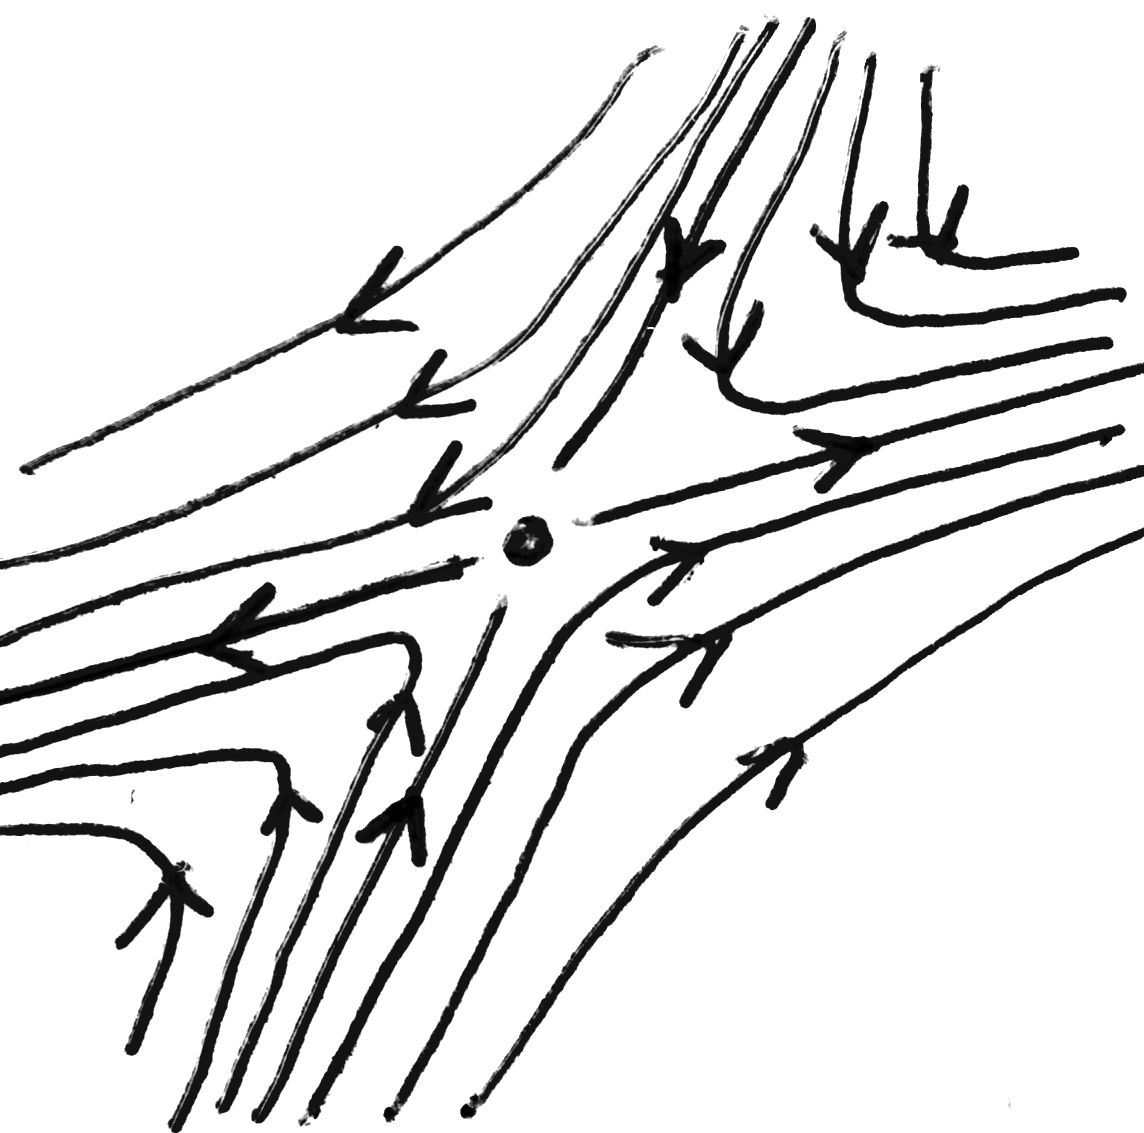
\includegraphics[width=0.75\textwidth]{sistemi_sella.png}
  \caption[1a]{sella (instabile)}
 \end{subfigure}
 \begin{subfigure}{5cm}
  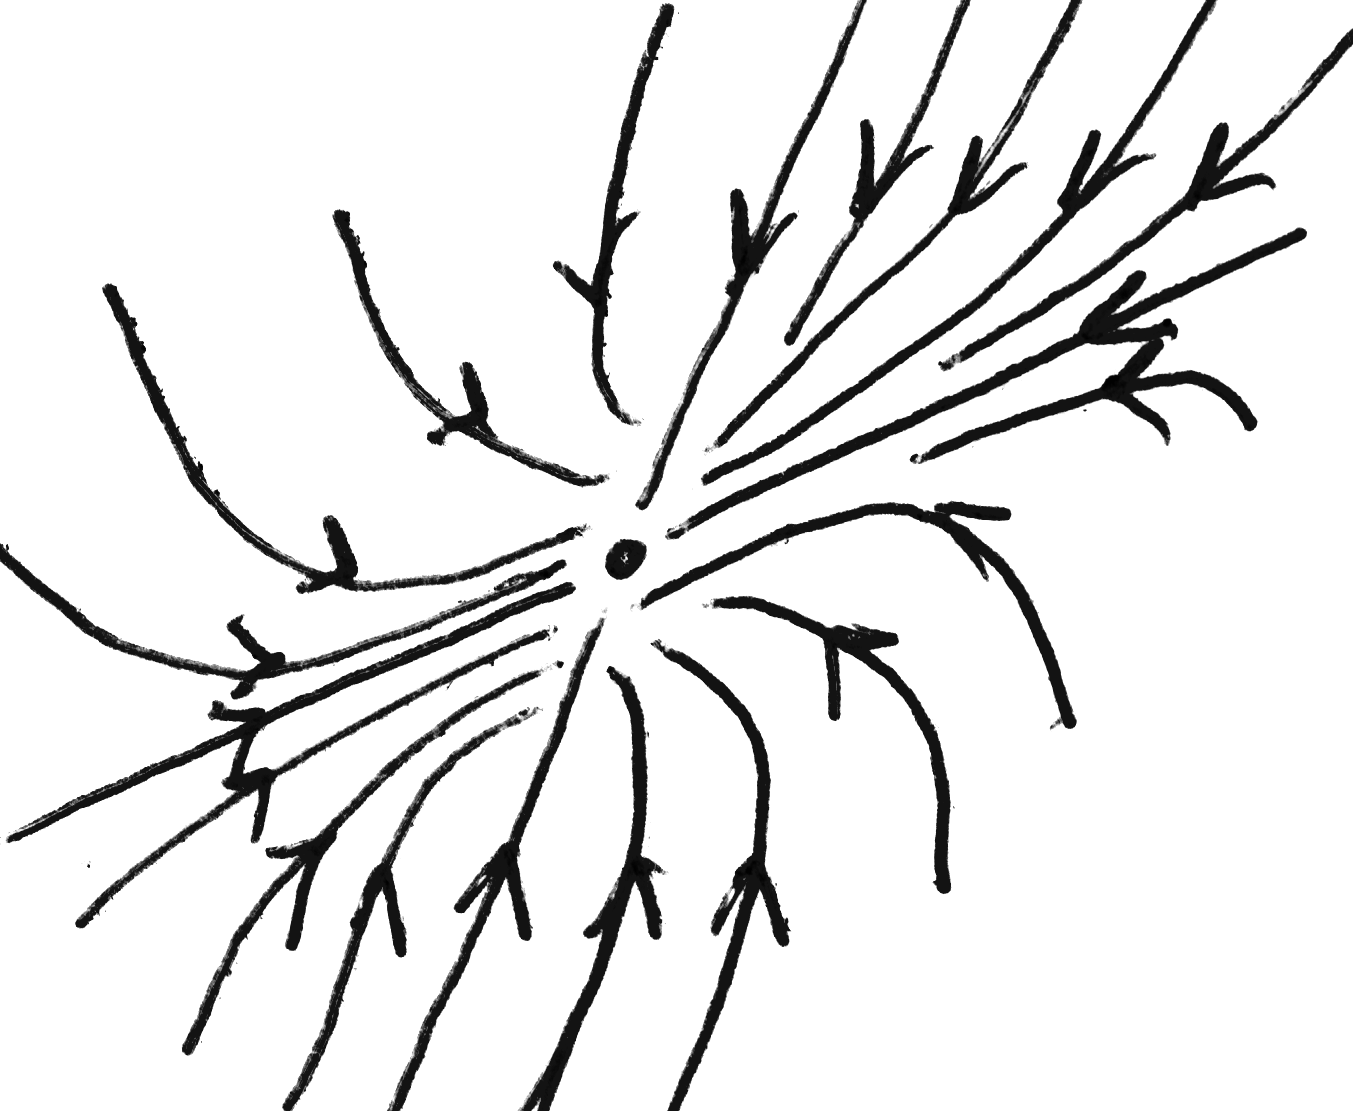
\includegraphics[width=0.75\textwidth]{sistemi_nodo.png}
  \caption{nodo stabile}
 \end{subfigure}
 \begin{subfigure}{5cm}
  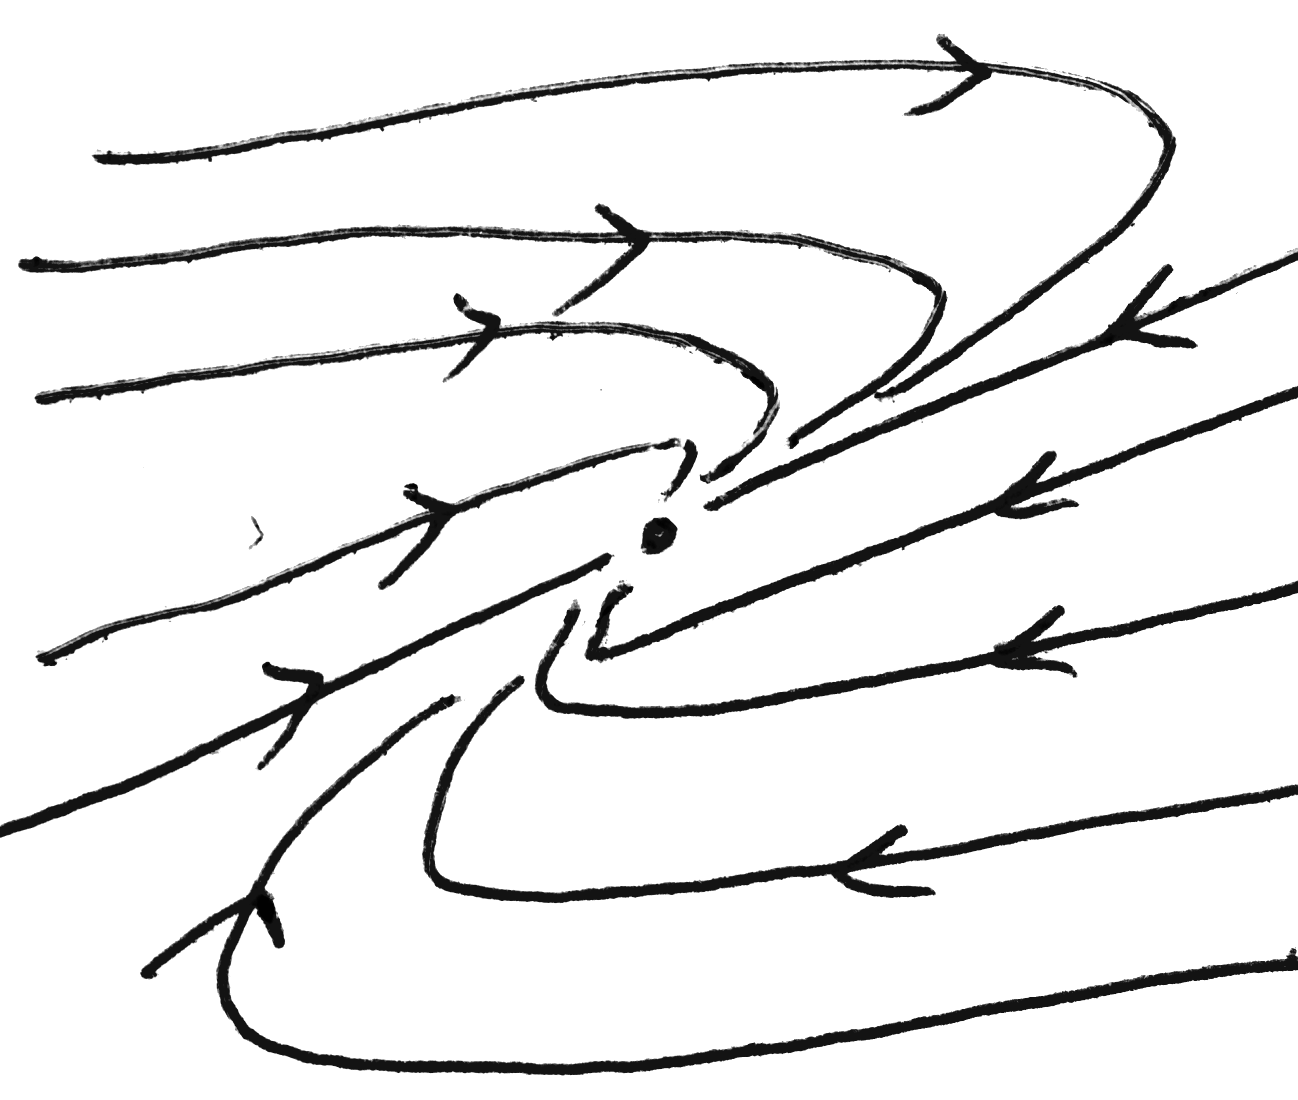
\includegraphics[width=0.75\textwidth]{sistemi_nodo_improprio.png}
  \caption{nodo improprio stabile}
 \end{subfigure}
 \begin{subfigure}{5cm}
  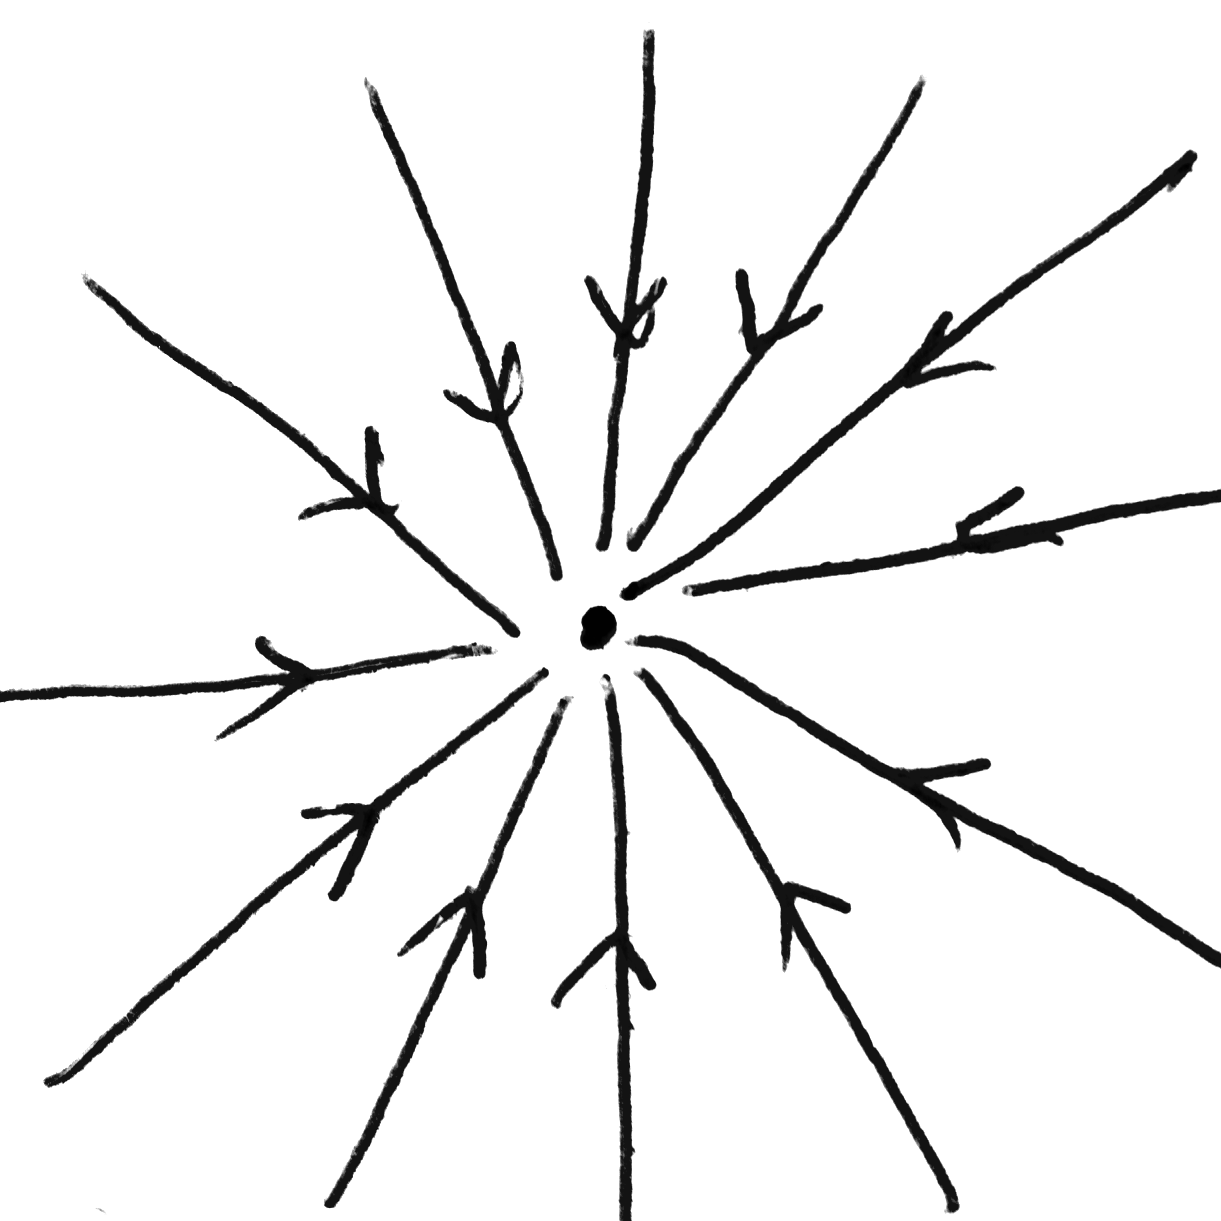
\includegraphics[width=0.75\textwidth]{sistemi_stella.png}
  \caption{stella stabile}
 \end{subfigure}
 \begin{subfigure}{5cm}
  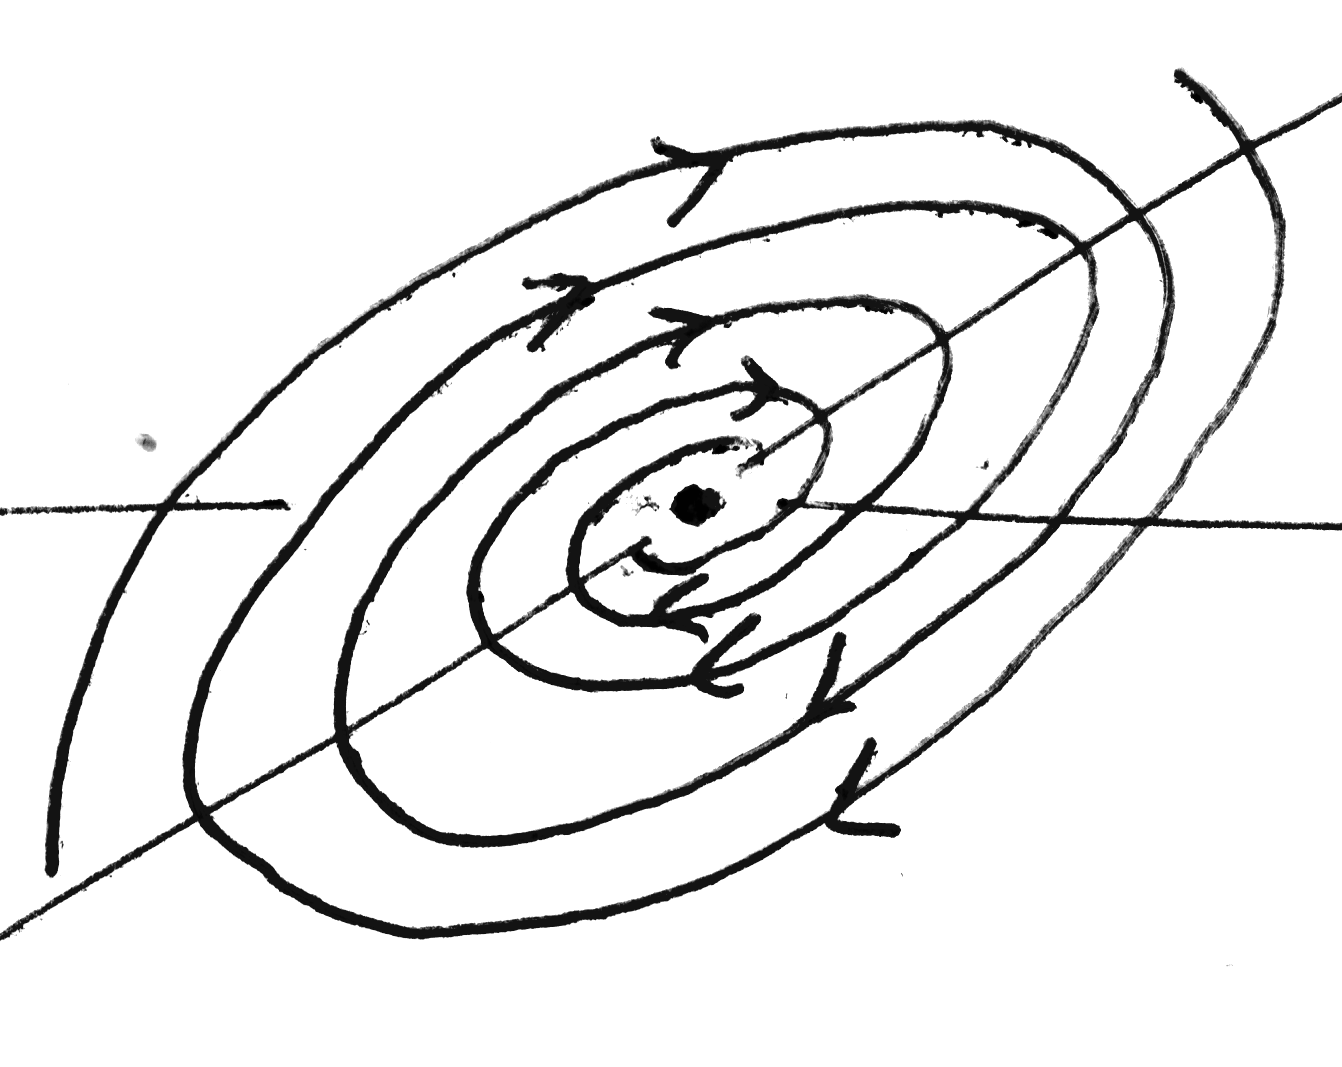
\includegraphics[width=0.75\textwidth]{sistemi_fuoco.png}
  \caption{fuoco stabile}
 \end{subfigure}
 \begin{subfigure}{5cm}
  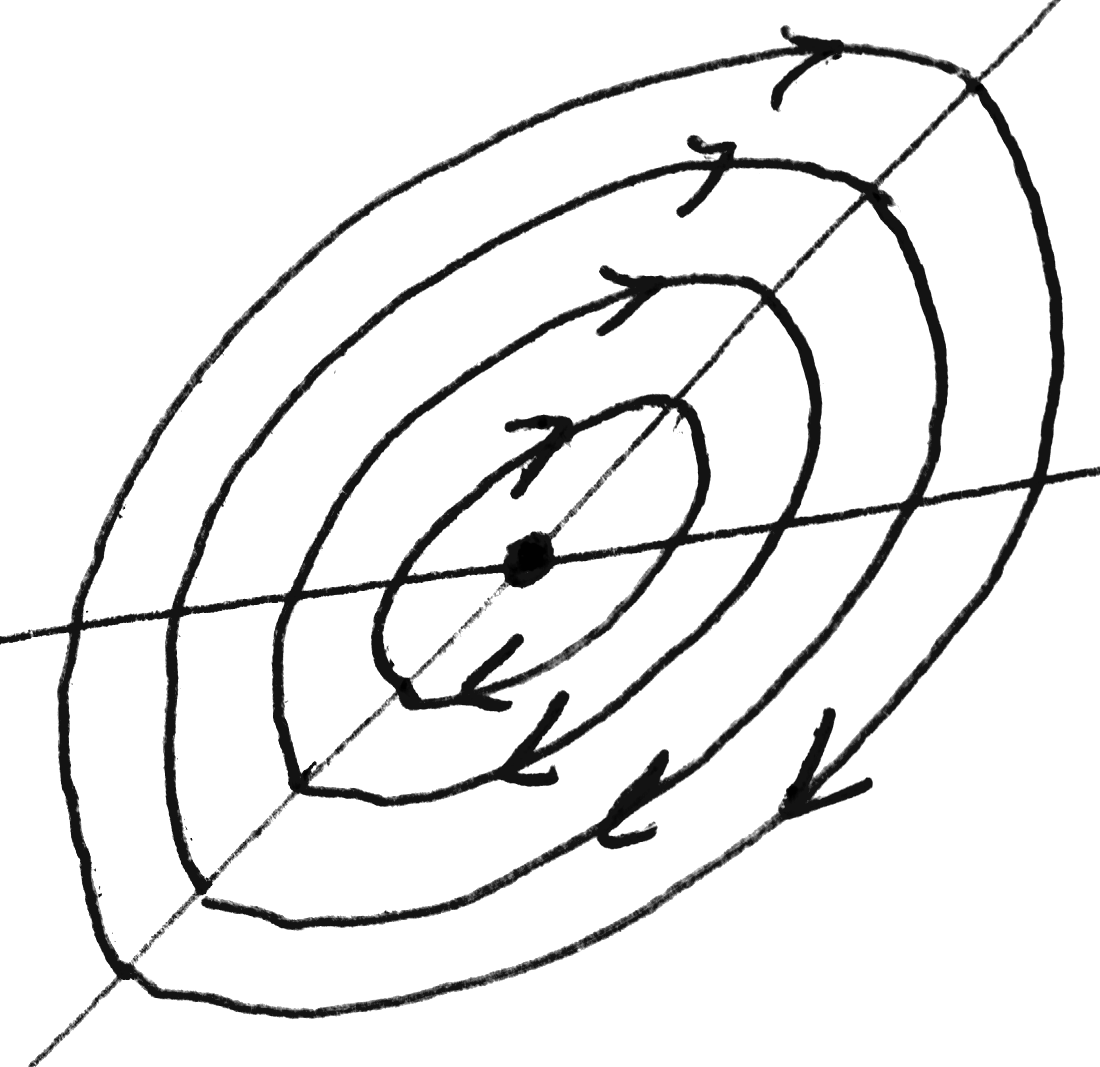
\includegraphics[width=0.75\textwidth]{sistemi_centro.png}
  \caption{centro (stabile)}
 \end{subfigure}
% \begin{caption}
% \qrcode{http://paolini.github.io/recurrence/ode.html?r=14.4&x=-0.375&y=0.447&points=0.363_0.19_1.28_0.789_2.39_1.3_3.5_1.76_-0.098_0.513_-0.467_1.39_-0.789_2.31_-1.02_3.55_-1.2_5.08_-1.16_6.69_-1.53_8.07_4.51_2.59_5.94_3.09_7.88_4.38_9.07_5.35_10.4_6.83_0.409_-0.593_1.05_-1.33_1.19_-2.48_1.33_-3.87_2.02_-5.2_2.16_-6.72_2.94_-7.74_-0.697_-0.0404_-1.34_-0.593_-2.63_-1.19_-3.6_-2.07_-5.35_-2.9_-7.06_-3.77_-8.53_-4.93_-10_-6.26_-3.74_9.04&fx=-2x%2By&fy=y%2B2x}
% \end{caption}
\end{figure}

Se i segni di $\lambda$ e $\mu$ sono opposti,
si ottiene una configurazione chiamata
\myemph{sella} (si veda figura).
Lungo l'autovettore con autovalore negativo
ci sarà convergenza verso l'origine, ma questa
convergenza è instabile in quanto ogni altra
curva tenderà invece a essere deviata
e a tendere asintoticamente verso la direzione
dell'autovettore con autovalore positivo.

Se $\lambda$ e $\mu$ sono entrambi negativi si
ha un \myemph{nodo stabile} in cui tutte le
curve convergono verso l'origine (soluzione
attrattiva). Se invece $\lambda$ e $\mu$
sono entrambi positivi le curve
saranno percorse in senso inverso e saranno
uscenti dall'origine: si avrà allora
un \myemph{nodo instabile}.

Se gli autovalori sono coincidenti $\lambda=\mu$
e se la matrice è diagonalizzabile allora
la matrice è diagonale, tutti i vettori sono
autovettori quindi in ogni direzione c'è
una traiettoria rettilinea.
La configurazione si
chiama \myemph{stella} (stabile o instabile a seconda
del segno negativo o positivo).

Se gli autovalori sono coincidenti $\lambda = \mu$ e la matrice
non è diagonalizzabile consideriamo l'autovettore (unico)
$\vec u$ con $A \vec u = \lambda \vec u$
e prendiamo un qualunque vettore $\vec w$
indipendente da $\vec u$. Allora si avrà
\[
  A \vec w = \alpha \vec u + \beta \vec w.
\]
Certamente $\alpha \neq 0$ altrimenti $\vec w$
sarebbe un autovettore e la matrice sarebbe diagonalizzabile.
Consideriamo allora $\vec v = \vec w / \alpha$
cosicché si ha $A \vec v = \vec u + \frac{\beta}{\alpha} \vec w$.
Nella base $\vec u, \vec v$ la matrice $A$ diventa
triangolare, e sulla diagonale troviamo i valori $\lambda$
e $\frac{\beta}{\alpha}$.
Ma allora $\frac{\beta}{\alpha} = \lambda$ in quanto sulla diagonale
abbiamo solo gli autovalori. Dunque se $X,Y$ sono le coordinate nel
sistema $\vec u, \vec v$, il sistema di equazioni diventa:
\[
\begin{cases}
X' = \lambda X + Y \\
Y' = \lambda Y.
\end{cases}
\]
Dalla seconda equazione si ottiene quindi $Y = a e^{\lambda t}$
con $a\in \RR$ costante arbitraria
e sostituendo nella prima si ottiene l'equazione
\[
  X' - \lambda X = a e^{\lambda t}
\]
che può essere risolta trovando una seconda costante arbitraria $b\in \RR$ e
\[
  X = (at+b) e^{\lambda t}.
\]
Se $a=0$ una traiettoria con $Y=0$ cioè nella direzione dell'unico autovettore.
Se $\lambda <0$ tale traiettoria sarà convergente a $0$ altrimenti sarà divergente.
Se $a\neq 0$ possiamo eliminare $t$ ponendo:
\[
  t = \frac 1 \lambda \ln \frac{Y}{a}
\]
e quindi
\[
  X = \enclose{\frac{a}{\lambda} \ln \frac{Y}{a}+ b} \frac{Y}{a}
  =  \frac{Y}{\lambda}\ln \frac{Y}{a}+ \frac{b}{a}Y.
\]
Studiando il grafico di questa funzione si ottengono qualitativamente
le curve disegnate in figura: la configurazione si chiama \myemph{nodo improprio}.
Come per i nodi le traiettorie convergono all'origine se $\lambda < 0$ e
divergono se $\lambda >0$.

Proviamo a trattare il caso, più interessante,
degli autovalori complessi. Se la matrice è a coefficienti
reali gli autovalori, quando
non reali, saranno certamente complessi coniugati:
\[
  \lambda = \alpha - i \beta,
  \qquad
  \mu = \alpha + i \beta
\]
con $\alpha,\beta\in \RR$, $\beta\neq 0$.

Sia $\vec v + i \vec w$ un autovettore complesso relativo
all'autovalore $\alpha - i \beta$.
Allora si ha
\[
 A\vec v + i A \vec w
 = A(\vec v + i \vec w)
 = (\alpha - i \beta)(\vec v + i \vec w)
 = \alpha \vec v + \beta \vec w +i(-\beta \vec v + \alpha \vec w).
\]
Uguagliando parte reale e parte immaginaria si trova
\[
  A \vec v = \alpha \vec v + \beta \vec w,
  \qquad
  A \vec w = -\beta \vec v + \alpha \vec w.
\]
A questo punto non è difficile verificare che $\vec v - i \vec w$
è un autovettore relativo all'autovalore coniugato $\alpha + i\beta$.
Visto che $\vec v\pm i\vec w$ sono due autovettori con autovalori
distinti sicuramente sono vettori indipendenti.
Dunque anche $\vec v$ e $\vec w$
(che si ottengono come multipli di somma e differenza)
sono vettori, stavolta reali
indipendenti.
Se $X,Y$ sono le coordinate nella base $\vec v$, $\vec w$, l'equazione
differenziale diventa:
\[
\begin{cases}
 X' = \alpha X - \beta Y \\
 Y' = \beta X + \alpha Y.
\end{cases}
\]
Si ha allora%
\footnote{Si potrebbe osservare che la matrice
$\begin{pmatrix}\alpha&-\beta\\ \beta & \alpha\end{pmatrix}$
è la matrice che rappresenta la moltiplicazione
complessa per il numero $\alpha + i\beta$. Dunque chiamando $Z=X+iY$
il sistema si potrebbe scrivere nella forma $Z'=(\alpha +i\beta)Z$
e si potrebbe quindi osservare immediatamente
che la soluzione deve essere della forma $Z = c e^{(\alpha+i\beta)t}$
con $c$ costante complessa. Ponendo poi $c=\rho e^{i\theta}$
si ottiene il risultato.}
\[
 X'' = \alpha X' - \beta Y'
 = \alpha X' - \beta (\beta X + \alpha Y)
\]
da cui, usando $\beta Y = \alpha X - X'$ possiamo eliminare la variabile $Y$
e ottenere una equazione del secondo ordine in $X$:
\[
 X'' = \alpha X' - \beta^2 X - \alpha (\alpha X - X')
  = 2 \alpha X' - (\alpha^2+\beta^2) X
\]
ovvero
\[
 X'' - 2 \alpha X' + (\alpha^2 + \beta^2) X = 0.
\]
Risolvendo questa equazione del secondo ordine ci si accorge
che le radici del polinomio caratteristico sono proprio $\alpha \pm i \beta$
e quindi le soluzioni si scrivono nella forma
\[
X = e^{\alpha t}(a \cos \beta t + b \sin \beta t)
\]
da cui
\begin{align*}
\beta Y
&= \alpha X - X'\\
& = \alpha e^{\alpha t}(a \cos \beta t + b \sin \beta t) \\
&\quad - \alpha e^{\alpha t}(a\cos \beta t + b \sin \beta t)
  - e^{\alpha t}(-\beta a \sin \beta t + b \beta \cos \beta t) \\
 &= \beta e^{\alpha t}(a\sin \beta t - b \cos \beta t).
\end{align*}
Dunque, ponendo $\rho=\sqrt{a^2+b^2}$ e scegliendo $\theta$
tale che $\cos \theta = \frac a \rho$ e $\sin \theta = - \frac b \rho$,
si ha
\[
  \begin{cases}
   X = \rho e^{\alpha t} \cos(\beta t + \theta),\\
   Y = \rho e^{\alpha t} \sin(\beta t + \theta).
  \end{cases}
\]
Se $\alpha \neq 0$ le traiettorie corrispondenti formano delle spirali
ellittiche che si avvitano nella direzione che porta il vettore $\vec v$ verso
il vettore $\vec w$. Se $\alpha < 0$ le spirali convergono verso l'origine del
sistema: avremo un \myemph{fuoco stabile}. Se $\alpha >0$ le orbite
divergono chiameremo la configurazione un \myemph{fuoco instabile}.
Se $\alpha = 0$ le traiettorie sono delle ellissi concentriche,
le soluzioni sono quindi periodiche e la configurazione
si chiama \myemph{centro}.

Se almeno uno dei due autovalori è nullo il comportamento del sistema è degenere,
si hanno delle soluzioni banali che non andremo a investigare.

\subsection{matrice esponenziale}

Per risolvere, in astratto, il sistema $n\times n$
\[
  \vec u' = A \vec u
\]
introduciamo le seguenti nozioni.

Sia $A$ una matrice quadrata $n\times n$. Definiamo la norma (norma
operatoriale) di $A$ come segue:
\[
  \Abs{ A } = \sup_{\abs{\vec v} \le 1} \abs{A\vec v}
\]
dove $\abs{ \vec v} = \sqrt{v_1^2+ \dots + v_n^2}$ è l'usuale norma del
vettore $\vec v\in \RR^n$.
Osserviamo che $\vec v\mapsto A\vec v$ è una funzione
continua e che $\ENCLOSE{\vec v\colon \abs{ \vec v} \le 1}$ è un insieme
compatto, dunque il $\sup$ nella definizione è in realtà un $\max$.

Per le proprietà del $\sup$ si ha:
\[
  \abs{A\vec v} \le \Abs{ A }\, \abs{ v }
\qquad\text{e}\qquad
  \Abs{ A B } \le \Abs{ A } \, \Abs{ B }.
\]
Dunque possiamo affermare il valore assoluto di ogni elemento di una
matrice si stima con la norma della matrice: $\abs{ A_{ij}} \le
\Abs{ A }$, infatti:
\[
  \abs{ A_{ij} } = \abs{ (A \vec e_j)_i} \le \abs{ A e_j}
  \le \Abs{ A }
\]
(dove $\vec e_j$ è il $j$-esimo vettore della base canonica di $\RR^n$).

Se $A_k$ è una successione di matrici, diremo che $A_k\to A$ se ogni
elemento della matrice $A_k$ converge al corrispondente elemento della
matrice $A$: $(A_k)_{ij} \to A_{ij}$. Questo corrisponde a considerare
la matrice $n\times n$ come un vettore dello spazio $\RR^{(n^2)}$.

Se $A(t)$ è una funzione a valori matrici (ovvero una matrice i cui
elementi sono funzioni di $t$), si potrà farne la derivata
come si fa per le funzioni vettoriali: $(A'(t))_{ij} = (A_{ij}(t))'$
cioè componente per componente. Le usuali regole per le derivate
valgono anche per le matrici, in particolare non è difficile
verificare (si espliciti la definizione del prodotto di matrici) che
\[
 (A(t)B(t))' = A'(t) B(t) + A(t) B'(t)
\]
dove, puntualizziamo, è importante mantenere i prodotti nell'ordine
giusto, in quanto il prodotto di matrici può non essere commutativo.

Se $A$ è una matrice quadrata, si definisce la matrice potenza $A^k$
per ogni $k$ naturale, mediante le proprietà
\[
  A^0 = I, \qquad A^{k+1} = A^kA.
\]
(se $A$ è invertibile si possono definire anche le potenze negative
$A^{-k}=(A^{-1})^k = (A^k)^{-1}$).

Definiamo allora la matrice esponenziale di $A$:
\[
  e^A = \sum_{k=0}^\infty \frac{A^k}{k!}.
\]
Per dare significato a questa definizione dobbiamo verificare che la
serie appena scritta sia convergente. Cioè dobbiamo verificare che per
ogni coppia di indici $ij$ sia convergente la serie numerica:
\[
 \sum_{k=0}^\infty \frac{(A^k)_{ij}}{k!}.
\]
Per quanto detto prima sappiamo che
$\abs{(A^k)_{ij}} \le \Abs{A^k} \le \Abs{A}^k$.
Dunque la serie in questione è
assolutamente convergente in quanto il suo valore assoluto si stima
con la serie
\[
 \sum_{k=0}^\infty \frac{\Abs{ A}^k}{k!} = e^{\Abs{ A}}
\]
che è convergente. La definizione della matrice $e^A$ è dunque
ben posta e si ha
\[
 \Abs{ e^A} \le e^{\Abs{ A }}.
\]

\begin{theorem}[proprietà dell'esponenziale matrice]
Siano $A$ e $B$ matrici quadrate $n\times n$ e $t$ uno scalare.
Valgono le seguenti proprietà:
\begin{enumerate}
\item $e^0 = I$ (dove $0$ è la matrice nulla $n\times n$ ed $I$ è la
  matrice identità con le stesse dimensioni);
\item se $AB=BA$ allora $e^A B = B e^A$;
\item $(e^{tA})' = A e^{tA}$;
\item $e^{-A} = (e^A)^{-1}$ (in particolare la matrice esponenziale è
  sempre invertibile);
\item se $\vec u(t)$ è una funzione a valori in $\RR^n$ che soddisfa
  l'equazione differenziale $\vec u'(t) = A\vec u(t)$ allora
  $\vec u(t) = e^{tA} \vec u(0)$;
\item se $AB=BA$ allora $e^{A+B} = e^A e^B$;
\item se $A$ è invertibile allora $e^{ABA^{-1}} = Ae^BA^{-1}$;
\item se $A$ è la matrice diagonale $A = \diag(\lambda_1, \dots, \lambda_n)$,
allora $e^A$
 è pure una matrice diagonale con $e^A = \diag(e^{\lambda_1},\dots, e^{\lambda_n})$;
\item se $A$ è una matrice triangolare con la diagonale nulla (cioè
  $A_{ij}=0$ se $i\ge j$) allora $e^A = \sum_{k=0}^n \frac{A^k}{k!}$
  (basta sommare i primi $n+1$ termini);
\item se $B$ è una matrice triangolare (cioè $B_{ij}=0$ se $i > j$)
  allora $B = D + A$ con $D$ matrice diagonale e $A$ matrice
  triangolare con la diagonale nulla e quindi $e^B = e^De^A$ si può
  calcolare riconducendosi ai punti precedenti.
\end{enumerate}
\begin{proof}
1. Per quanto riguarda $e^0$ osserviamo che per definizione $0^0=I$
mentre $0^k=0$ se $k>0$. Dunque direttamente dalla definizione si
ottiene $e^0=I$.

2. Se $AB=BA$ osserviamo che si ha anche $A^k B=B A^k$ (la matrice $B$
commuta con ogni fattore del prodotto $A^k$). Dunque:
\[
 \sum_{k=0}^N \frac{A^k}{k!} B = B \sum_{k=0}^N \frac{A^k}{k!}
\]
e passando al limite $N\to \infty$ si ottiene $e^A B = B e^A$.

3. Per calcolare la derivata di $e^{tA}$ vogliamo dimostrare che la serie
che definisce $e^{tA}$ converge totalmente quando $t$ varia in un
qualunque intervallo limitato. Poniamo allora $t\in [-M,M]$. Si ha:
\[
  \sup_{t\in[-M,M]}\frac{\Abs{ (tA)^k}}{k!}
  = \sup_{t\in[-M,M]}\frac{\abs{ t}^k \Abs{ A^k}}{k!}
  \le \frac{M^k\Abs{ A}^k}{k!}
\]
la cui serie è convergente qualunque sia $M\in \RR$. Dunque la serie
che definisce $e^{tA}$ è una serie di funzioni continue e derivabili
che converge totalmente su ogni intervallo limitato. Possiamo quindi
derivare la serie termine a termine:
\[
(e^{tA})' = \sum_{k=0}^\infty \frac{((tA)^k)'}{k!}
 = \sum_{k=1}^\infty \frac{kt^{k-1} A^k}{k!}
 = A \sum_{k=1}^\infty \frac{t^{k-1}A^{k-1}}{(k-1)!}
 = A e^{tA}.
\]

4. Dimostriamo ora che $U(t) = e^{tA}e^{-tA}=I$ per ogni $t$. Si ha:
\[
 U'(t) = A e^{tA}e^{-tA} + e^{tA}(-A)e^{-tA}
       = A e^{tA}e^{-tA} - A e^{tA}e^{-tA} = 0
\]
($Ae^{tA} = e^{tA}A$ in quanto $A$ e $tA$ commutano).
Dunque $U'(t)=0$ cioè $U(t)$ è costante ovvero $U(t)=U(0)$. Ma $U(0)=I$
in quanto $e^0=I$ e quindi $U(t)=I$ per ogni $t$.

5. Prendiamo l'equazione $\vec u' = A\vec u$, moltiplicando a sinistra per
$e^{-tA}$ l'equazione diventa
$e^{-tA} \vec u' - e^{-tA} A \vec u=0$ cioè $(e^{-tA} \vec u)' = 0$. Questo significa
che la funzione $e^{-tA}\vec u = c$ costante e moltiplicando a sinistra per
$e^{tA}$ si ottiene dunque $\vec u = e^{tA}c$ come volevasi dimostrare.

6. Per dimostrare la proprietà $e^{A+B}=e^A e^B$ consideriamo la quantità
$U(t) = e^{-t(A+B)} e^{tA} e^{tB}$. Se dimostriamo che $U$ è costante,
visto che $\vec u(0)=I$ si avrà anche $U(1)=I$ che è equivalente a quanto
vogliamo dimostrare. Dunque verifichiamo che la derivata è nulla,
sfruttando l'ipotesi $AB=BA$ che ci permette di far commutare i prodotti:
\begin{align*}
U'(t) & = -(A+B)e^{-t(A+B)} e^{tA} e^{tB} + e^{-t(A+B)}Ae^{tA}e^{tB} +
e^{-t(A+B)}e^{tA} B e^{tB} \\
& = [-(A+B) + A + B] U(t) = 0.
\end{align*}

7. Se $A$ è invertibile allora $(ABA^{-1})^k = ABA^{-1}ABA\dots ABA^{-1}
= AB^k A^{-1}$. Dunque nelle somme parziali della serie che definisce l'esponenziale
$e^{ABA^{-1}}$ si può raccogliere $A$ a sinistra e $A^{-1}$ a destra e
al centro rimane la serie che definisce $e^B$.

8. Se la matrice $A$ è diagonale con $A_{ii}=\lambda_i$ allora $A^k$
risulta essere una matrice diagonale con $(A^k)_{ii} =
\lambda_i^k$. Dunque nella definizione di esponenziale $e^A$ i termini
della serie sono tutte matrici diagonali, e sulla diagonale compare la
serie che definisce l'esponenziale $e^{\lambda_i}$.

9. Se $A$ è una matrice triangolare con $A_{ij}=0$ quando $i\ge j$, si
osserva che $A^2$ avrà degli zeri anche sopra la diagonale:
$(A^2)_{ij}=0$ quando $i+1\ge j$ (si applichi la definizione di
prodotto, riga per colonna). Nelle moltiplicazioni successive $A^3,
A^4,\dots$ si aggiungerà sempre una diagonale di zeri finché la matrice non
si annulla completamente $A^n=0$. Dunque la serie che definisce $e^A$
contiene solo un numero finito di termini (i primi $n+1$) e può essere
calcolata esplicitamente.

10. L'ultima proprietà è una osservazione che non richiede dimostrazione.
\end{proof}
\end{theorem}
